% Options for packages loaded elsewhere
\PassOptionsToPackage{unicode}{hyperref}
\PassOptionsToPackage{hyphens}{url}
%
\documentclass[
]{book}
\usepackage{amsmath,amssymb}
\usepackage{lmodern}
\usepackage{iftex}
\ifPDFTeX
  \usepackage[T1]{fontenc}
  \usepackage[utf8]{inputenc}
  \usepackage{textcomp} % provide euro and other symbols
\else % if luatex or xetex
  \usepackage{unicode-math}
  \defaultfontfeatures{Scale=MatchLowercase}
  \defaultfontfeatures[\rmfamily]{Ligatures=TeX,Scale=1}
\fi
% Use upquote if available, for straight quotes in verbatim environments
\IfFileExists{upquote.sty}{\usepackage{upquote}}{}
\IfFileExists{microtype.sty}{% use microtype if available
  \usepackage[]{microtype}
  \UseMicrotypeSet[protrusion]{basicmath} % disable protrusion for tt fonts
}{}
\makeatletter
\@ifundefined{KOMAClassName}{% if non-KOMA class
  \IfFileExists{parskip.sty}{%
    \usepackage{parskip}
  }{% else
    \setlength{\parindent}{0pt}
    \setlength{\parskip}{6pt plus 2pt minus 1pt}}
}{% if KOMA class
  \KOMAoptions{parskip=half}}
\makeatother
\usepackage{xcolor}
\usepackage{longtable,booktabs,array}
\usepackage{calc} % for calculating minipage widths
% Correct order of tables after \paragraph or \subparagraph
\usepackage{etoolbox}
\makeatletter
\patchcmd\longtable{\par}{\if@noskipsec\mbox{}\fi\par}{}{}
\makeatother
% Allow footnotes in longtable head/foot
\IfFileExists{footnotehyper.sty}{\usepackage{footnotehyper}}{\usepackage{footnote}}
\makesavenoteenv{longtable}
\usepackage{graphicx}
\makeatletter
\def\maxwidth{\ifdim\Gin@nat@width>\linewidth\linewidth\else\Gin@nat@width\fi}
\def\maxheight{\ifdim\Gin@nat@height>\textheight\textheight\else\Gin@nat@height\fi}
\makeatother
% Scale images if necessary, so that they will not overflow the page
% margins by default, and it is still possible to overwrite the defaults
% using explicit options in \includegraphics[width, height, ...]{}
\setkeys{Gin}{width=\maxwidth,height=\maxheight,keepaspectratio}
% Set default figure placement to htbp
\makeatletter
\def\fps@figure{htbp}
\makeatother
\setlength{\emergencystretch}{3em} % prevent overfull lines
\providecommand{\tightlist}{%
  \setlength{\itemsep}{0pt}\setlength{\parskip}{0pt}}
\setcounter{secnumdepth}{5}
\usepackage{booktabs}
\usepackage{amsthm}
\makeatletter
\def\thm@space@setup{%
  \thm@preskip=8pt plus 2pt minus 4pt
  \thm@postskip=\thm@preskip
}
\makeatother
\ifLuaTeX
  \usepackage{selnolig}  % disable illegal ligatures
\fi
\usepackage[]{natbib}
\bibliographystyle{apalike}
\IfFileExists{bookmark.sty}{\usepackage{bookmark}}{\usepackage{hyperref}}
\IfFileExists{xurl.sty}{\usepackage{xurl}}{} % add URL line breaks if available
\urlstyle{same} % disable monospaced font for URLs
\hypersetup{
  pdftitle={Introduction to Freight Transportation},
  pdfauthor={Scott S. Washburn, University of Florida, https://swash.essie.ufl.edu; Evangelos Kaiser, Florida Atlantic University, http://www.eng.fau.edu/directory/faculty/kaisar/; Lili Du, University of Florida, https://www.essie.ufl.edu/people/name/lili-du/},
  hidelinks,
  pdfcreator={LaTeX via pandoc}}

\title{Introduction to Freight Transportation}
\author{Scott S. Washburn, University of Florida, \url{https://swash.essie.ufl.edu} \and Evangelos Kaiser, Florida Atlantic University, \url{http://www.eng.fau.edu/directory/faculty/kaisar/} \and Lili Du, University of Florida, \url{https://www.essie.ufl.edu/people/name/lili-du/}}
\date{2023-08-04}

\begin{document}
\maketitle

{
\setcounter{tocdepth}{1}
\tableofcontents
}
\hypertarget{preface}{%
\chapter{Preface}\label{preface}}

This material is intended for an introduction to freight transportation course.Initial development of this material was sponsored by the Freight Mobility Research Institute (\url{http://eng.fau.edu/research/fmri/}).

An example figure is shown in Figure \ref{fig:PortImage}

\begin{figure}

{\centering \includegraphics[width=0.9\linewidth]{./Images/PortOfMiami} 

}

\caption{Port of Miami Partial Schematic}\label{fig:PortImage}
\end{figure}

\hypertarget{intro}{%
\chapter{Introduction}\label{intro}}

The movement of freight is a key foundation to the functioning of our society and economy.

\hypertarget{intro-agencies}{%
\section{Applicable Federal Agencies}\label{intro-agencies}}

\begin{itemize}
\tightlist
\item
  BTS - Bureau of Transportation Statistics (\url{https://www.bts.gov/})
\item
  FHWA - Federal Highway Administration (\url{https://www.fhwa.dot.gov/})
\item
  FMCSA - Federal Motor Carrier Safety Administration (\url{https://www.fmcsa.dot.gov/})
\item
  NHTSA - National Highway Traffic Safety Administration (\url{https://www.nhtsa.gov/})
\item
  USDOT - United States Department of Transportation (\url{https://www.transportation.gov/})
\end{itemize}

\hypertarget{intro-statistics}{%
\section{Freight movement statistics}\label{intro-statistics}}

\begin{enumerate}
\def\labelenumi{\arabic{enumi})}
\item
  Mobility refers to the ease that a passenger or a freight unit can move across a transportation system. High mobility requires limited efforts, while low mobility is related to complexity and high costs.
\item
  For freight,mobility is cargo-dependent, with some commodities having limited storage requirements but heavy to carry.
\end{enumerate}

\textbf{Weight of shipments by transportation mode}

\begin{figure}

{\centering 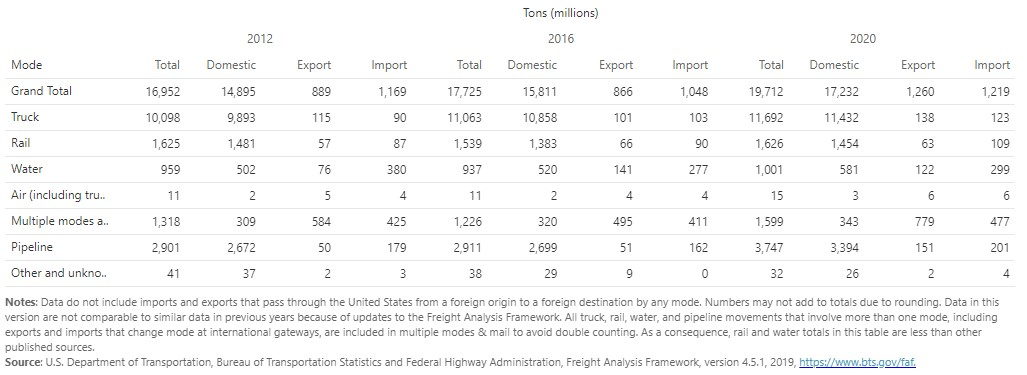
\includegraphics{./Images/FreightShipments_Weight} 

}

\caption{Weight of shipments by transportation mode}\label{fig:FreightByWeightImage}
\end{figure}

\textbf{Value of shipments by transportation mode}

\begin{figure}

{\centering 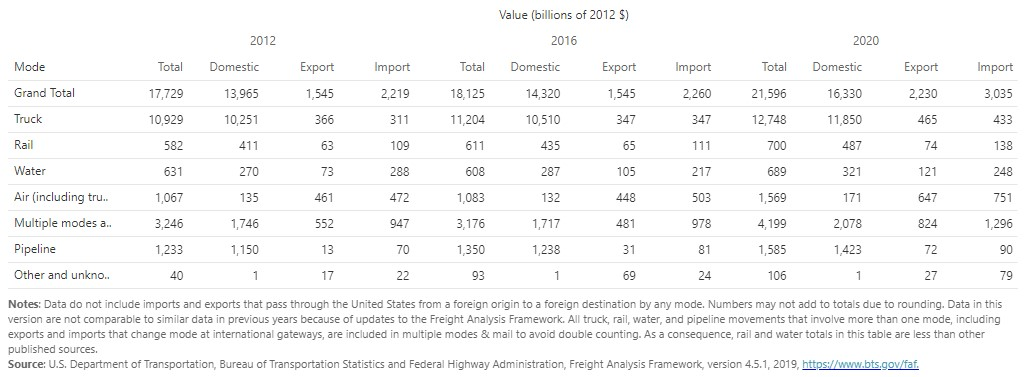
\includegraphics{./Images/FreightShipments_Value} 

}

\caption{Value of shipments by transportation mode}\label{fig:FreightByValueImage}
\end{figure}

Reference BTS

\hypertarget{intro-Freight}{%
\section{Freight Transportation}\label{intro-Freight}}

\begin{enumerate}
\def\labelenumi{\arabic{enumi})}
\item
  The figure 2.3 shows the Ton-Miles of Freight transported by different transportation modes.
\item
  Truck remains the premiere mode of freight transportation through the past two decades.
\item
  Further growth in the future with advancements in electric vehicles and automation.
\item
  Other modes are meanwhile holding relatively stable throughout the years.
\item
  Freight transportation movements are expected to increase over the next few decades as global populations grow and consumer spending power increases.
\item
  The freight transportation system in the United States includes an extensive network of highways, railroads, waterways, pipelines, and airways: 958,000 miles of Federal-aid highways, 141,000 miles of railroads, 11,000 miles of inland waterways, and 1.6 million miles of pipelines.
\item
  Figure 2.4 shows historical and forecasted mode share in ton-miles from 1990--2040.
\item
  The data reveal that most freight transportation modes are expected to experience increased volumes, although the amount of expected growth will vary by mode, with pipelines projected to have negative growth to year 2040.
\end{enumerate}

\begin{figure}

{\centering 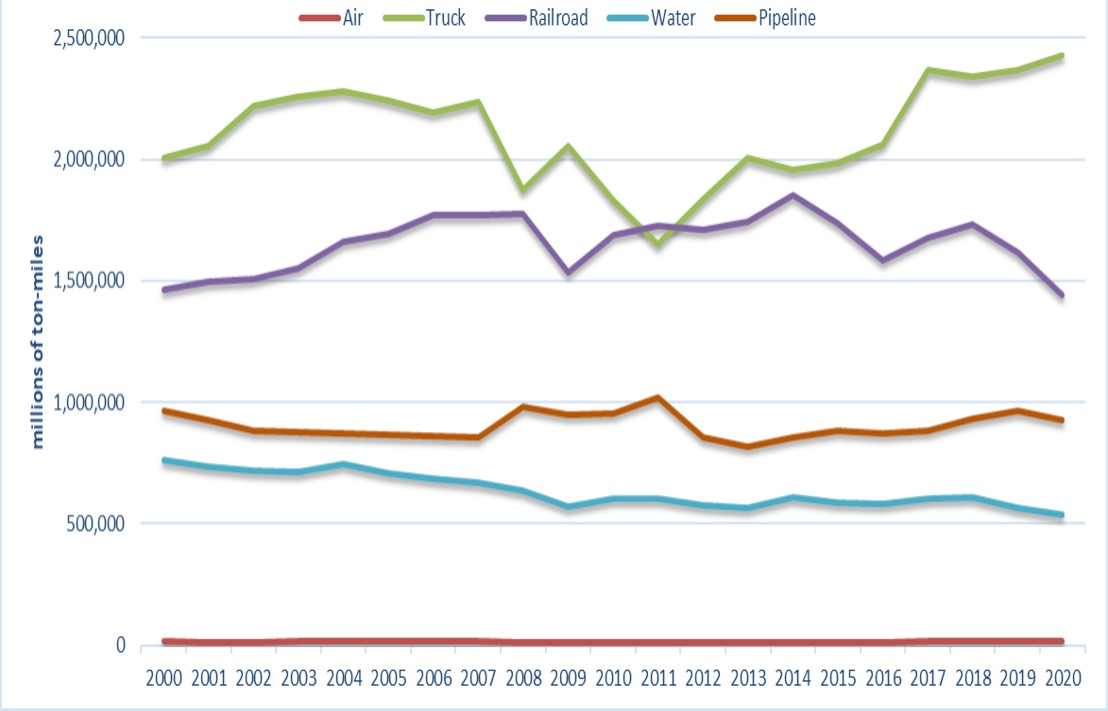
\includegraphics{./Images/Intro/U.S. Ton-Miles of Freight} 

}

\caption{U.S. Ton-Miles of Freight}(\#fig:Figure 2.3)
\end{figure}

Source: \url{https://www.bts.gov/content/us-ton-miles-freight}

\begin{figure}

{\centering \includegraphics{./Images/Intro/Historical and Forecasted Mode Share of Ton-miles, 1990–2040} 

}

\caption{Historical and Forecasted Mode Share of Ton-miles, 1990–2040}(\#fig:Figure 2.4)
\end{figure}

Source: 2016 Freight Quick Facts Report, DOT, Draft National Freight Strategic Plan, BTS Special Tabulation

\hypertarget{ntro-Freight_Index}{%
\section{Freight Transportation Service Index}\label{ntro-Freight_Index}}

\begin{enumerate}
\def\labelenumi{\arabic{enumi})}
\item
  The Freight Transportation Services Index, an indicator of monthly changes in freight carried by for-hire transportation companies.
\item
  Not exactly paralleled the demand for consumer goods since August 2019.
\item
  The volume of freight moved declined moderately from August 2019 through February 2020, then collapsed with the arrival of COVID-19 in March but quickly rebounded by summer.
\end{enumerate}

\begin{figure}

{\centering \includegraphics{./Images/Intro/Freight Transportation Services Index 2016–2021} 

}

\caption{Freight Transportation Services Index 2016–2021}(\#fig:Figure 2.5)
\end{figure}

\hypertarget{intro-Freight_economy}{%
\section{Freight Transportation and the Economy}\label{intro-Freight_economy}}

\begin{enumerate}
\def\labelenumi{\arabic{enumi})}
\item
  The benefits of freight transportation to the economy are enormous.
\item
  Freight transportation increases the value of goods by moving them to locations where they are worth more and encourages competition and production.
\item
  Freight transportation also stimulates demand for goods and services and employs millions of people.
\item
  Freight transportation infrastructure is a significant component of our nation's wealth and productive capacity.
\item
  From a macroeconomic perspective, transportation accounts for a significant share of the U.S. GDP. In 2000, purchases of transportation-related goods and services accounted for approximately 11 percent of GDP (USDOT BTS 2002).
\item
  Only housing, health care, and food accounted for a greater share. For-hire transportation services, which include warehousing, contributed about 3.3 percent (\$303 billion) to GDP.
\item
  Many industries and businesses depend on their own transportation operations (primarily trucking) to move goods. These ``in-house'' transportation services contributed an additional \$142 billion to the economy (USDOT BTS 2001b).
\item
  Freight transportation also contributes to the economy by providing jobs to millions of people---an important indicator of economic growth.
\item
  In 2000, more than 10 million people were employed in transportation-related industries, including for-hire services, vehicle manufacturing, and parts suppliers.
\item
  For-hire transportation (including warehousing) employed more than 4.4 million workers, a majority of whom worked in freight-related jobs.
\item
  Another 5.5 million people worked in transportation occupations in non transportation industries, such as truck drivers for grocery stores (USDOT BTS 2001b).
\item
  Truck drivers, alone, accounted for nearly 70 percent of the total number of transportation occupational workers (USDOT BTS 2002b).
\item
  Improvements in freight productivity help the United States maintain its competitive position in the world economy.
\item
  The Bureau of Labor Statistics reports that productivity for the intercity trucking, railroad, air transport, and petroleum pipeline industries has improved over the last 20 years.
\end{enumerate}

\hypertarget{intro-Freight_movement}{%
\section{Growing Freight Movement}\label{intro-Freight_movement}}

\begin{enumerate}
\def\labelenumi{\arabic{enumi})}
\item
  Improvements in railroad productivity resulted primarily from deregulation, divestiture of uneconomic lines, reductions in the labor force, and changes in technology and logistics. Productivity improvements in trucking resulted primarily from public investments in a high-quality national road network and deregulation.
\item
  The volume of freight moved by the U.S. transportation system has grown dramatically in recent decades and is projected to increase nearly 70 percent by 2020.
\item
  The liberalization of trade policies, such as the North American Free Trade Agreement (NAFTA), internationalization of supply chains, and changes in transportation and information technologies have contributed to this increase in freight movement.
\item
  As a share of the gross domestic product (GDP), U.S. exports and imports grew from 9 percent in 1960 to 23 percent in 2002. U.S. international trade is forecast to reach 37 percent of GDP by 2025.
\item
  Trucks carried about 71 percent of all tonnage and 80 percent of the value of U.S. shipments in 1998.
\item
  Even with growth in airfreight, maritime, and rail services, the percentage of urban interstates carrying more than 10,000 trucks daily is expected to increase from 27 percent in 1998 to 69 percent in 2020.
\item
  In recent years, trade growth has increased the number of commercial vehicles on U.S. roadways and, indirectly, the potential demand for more productive and larger commercial trucks. Trucks move a majority of freight tonnage.
\item
  In 2002, 7.9 million large trucks (trucks with six or more tires) were on the road, compared with 6.2 million in 1990, and trucks contributed to 7.5 percent of all vehicle miles traveled in 2002.
\item
  Trucks transported the vast majority of freight by both weight and value in 2018 (68\% and 73\%, respectively). While pipelines and rail together accounted for over 25\% of freight tonnage, they accounted for just over 12\% of freight value. Domestic freight movement in 2018 totaled 16.5 billion tons with a total value of \$14.8 billion.
\end{enumerate}

\begin{figure}

{\centering 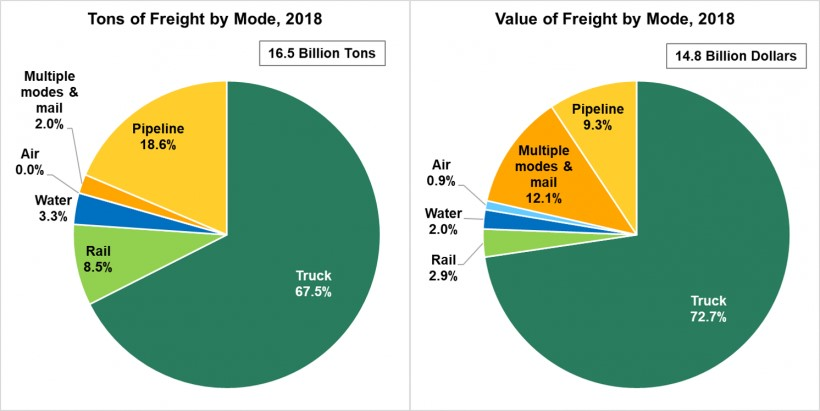
\includegraphics{./Images/Intro/Freight by Mode, 2018} 

}

\caption{Freight by Mode, 2018}(\#fig:Figure 2.6)
\end{figure}

Source:U.S. Department of Transportation,Freight Analysis Framework, Version 4.5.1, December 2019. Data Tabulation Tool queried July 2, 2020.

\hypertarget{intro-Freight_mobility}{%
\section{Freight Mobility and Statistics}\label{intro-Freight_mobility}}

\begin{figure}

{\centering 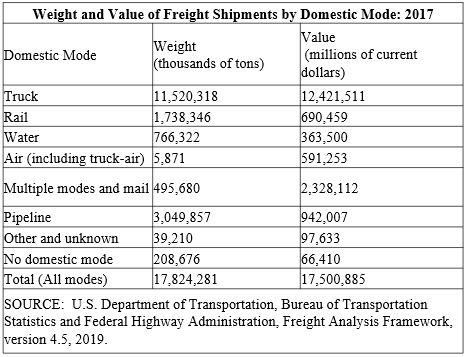
\includegraphics{./Images/Intro/Weight and Value Freight Shipments by Domestic Mode- 2017} 

}

\caption{Weight and Value Freight Shipments by Domestic Mode- 2017}(\#fig:Figure 2.7)
\end{figure}

\begin{figure}

{\centering 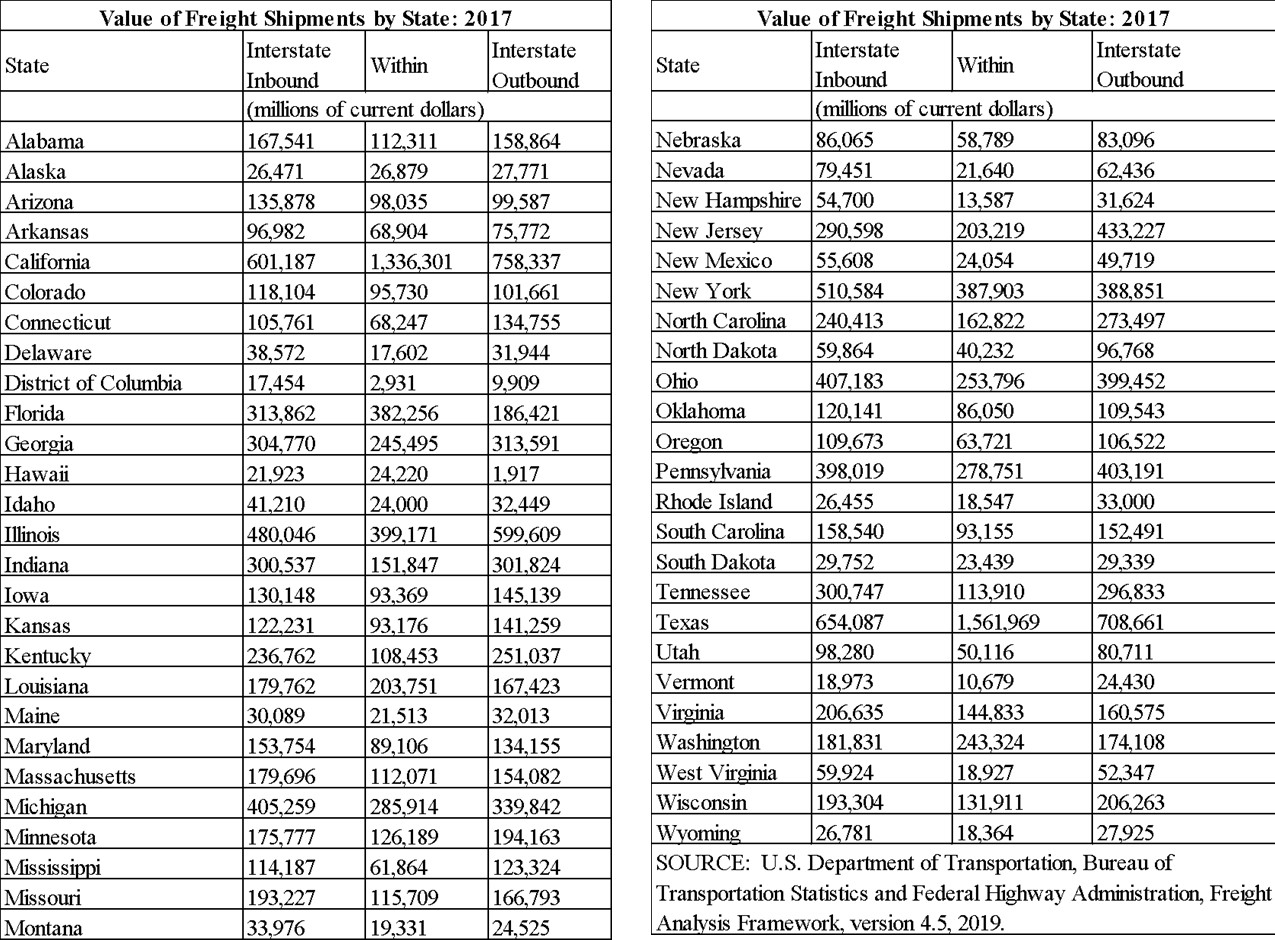
\includegraphics{./Images/Intro/Value of Freight Shipments by State- 2017} 

}

\caption{Value of Freight Shipments by State- 2017}(\#fig:Figure 2.8)
\end{figure}

\hypertarget{intro-Mode_Share}{%
\section{Freight Mobility and Statistics}\label{intro-Mode_Share}}

The modal distribution for ton-miles is similar to that for tons, with the exception of long-distance water moves. Rail moved nearly two-thirds of total ton-miles while pipelines accounted for 70 percent of ton-miles over distances more than 1,000 miles.

\begin{figure}

{\centering 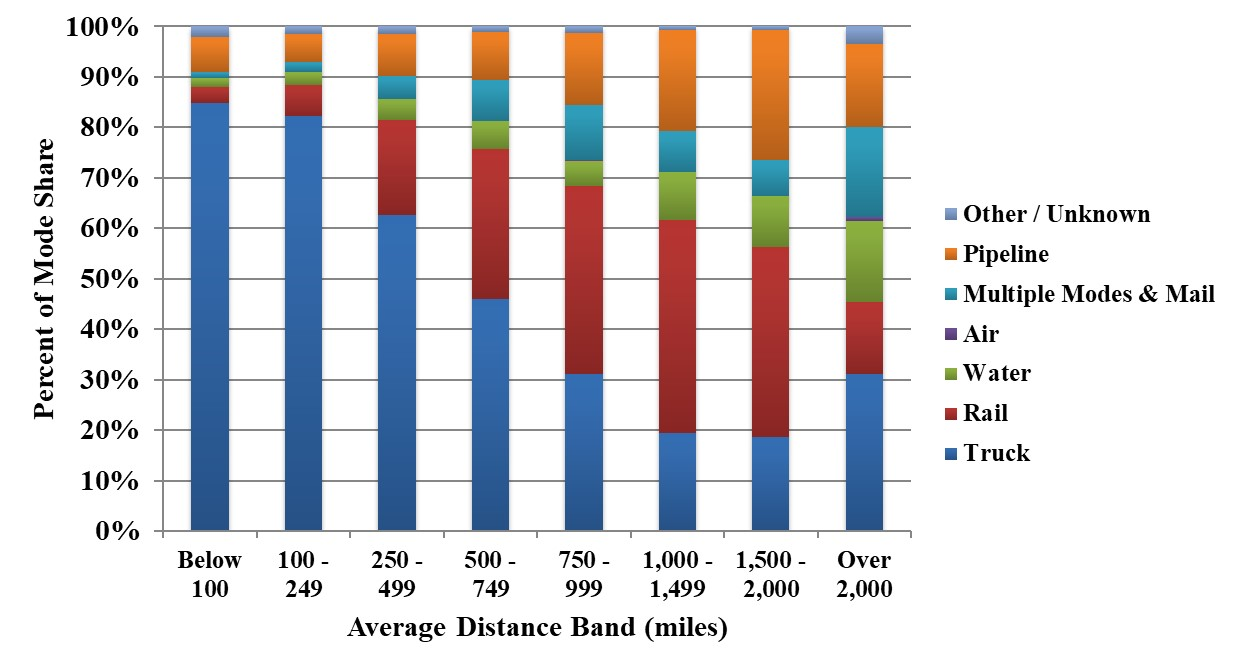
\includegraphics{./Images/Intro/Mode Share of Freight Ton-Miles by Distance Band-2007} 

}

\caption{Mode Share of Freight Ton-Miles by Distance Band-2007}(\#fig:Figure 2.9)
\end{figure}

\begin{figure}

{\centering 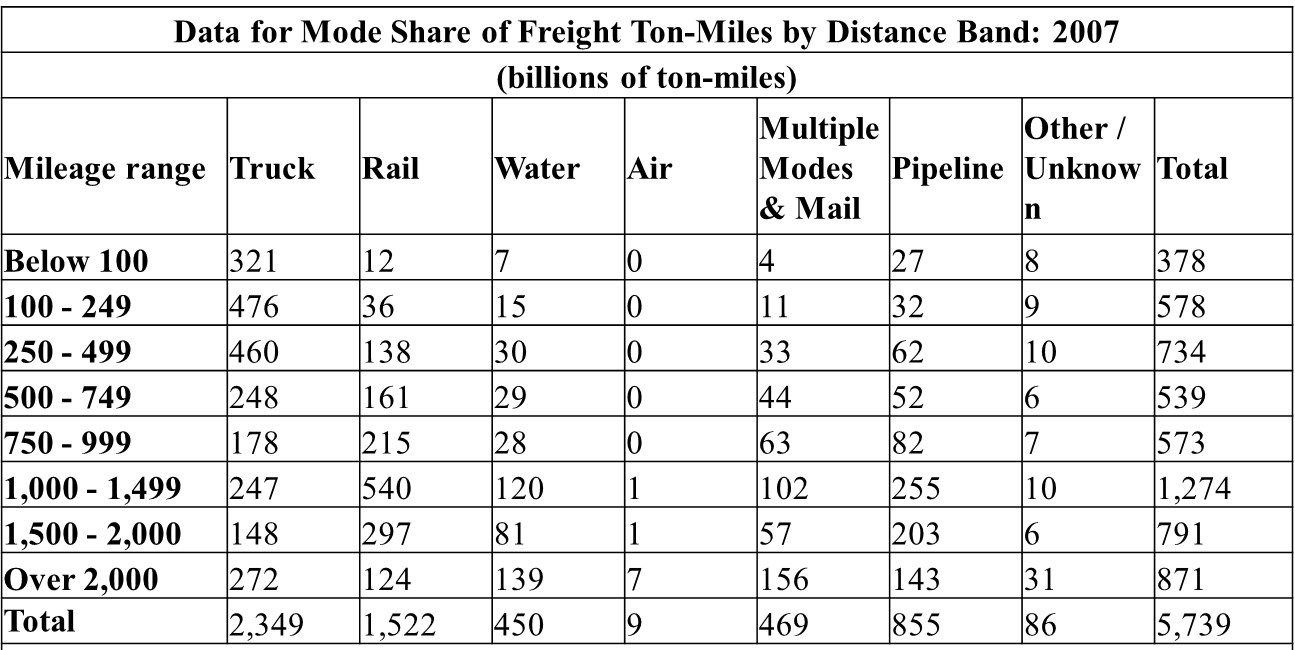
\includegraphics{./Images/Intro/Data for Mode Share of Freight Ton-Miles by Distance Band- 2007} 

}

\caption{Data for Mode Share of Freight Ton-Miles by Distance Band- 2007}(\#fig:Figure 2.10)
\end{figure}

Source: U.S. Department of Transportation, Federal Highway Administration, Office of Freight Management and Operations, Freight Analysis Framework, version 3.4, 2012.

\hypertarget{intro-Goods_Volume}{%
\section{Goods Volume/ Value Coming Into/ Out Various Sea Ports}\label{intro-Goods_Volume}}

Outlines:

\begin{enumerate}
\def\labelenumi{\arabic{enumi})}
\item
  Sea Port Function
\item
  Top 25 Tonnage Ports in 2020
\item
  The busiest container ports in the United States
\item
  Sea port goods movement
\item
  Container Sea Ports
\item
  Container Terminal Structure
\item
  Goods movement in Seaport
\item
  Sea-port Logistic
\end{enumerate}

\hypertarget{intro-Sea_Port_Function}{%
\section{Sea Port}\label{intro-Sea_Port_Function}}

\begin{enumerate}
\def\labelenumi{\arabic{enumi})}
\item
  Ports can serve a range of vessels including recreational watercraft, barges, ferries, and ocean-going cargo and passenger ships. The United States has over 150 deep-draft ports, which serve ocean-going ships.
\item
  Seaports are maritime facilities that can comprise one or more wharves where ships can dock to load and discharge cargo and passengers.
\item
  Since the dawn of commerce, people have been using boxes, sacks, barrels and containers of varying sizes to transport goods over long distances.
\item
  Now, an estimated 90\% of the world's goods are transported by sea.
\item
  The average size of a container ship has doubled in the past 20 years alone, with the largest ships sailing today capable of hauling 24,000 containers.
\end{enumerate}

\begin{figure}

{\centering 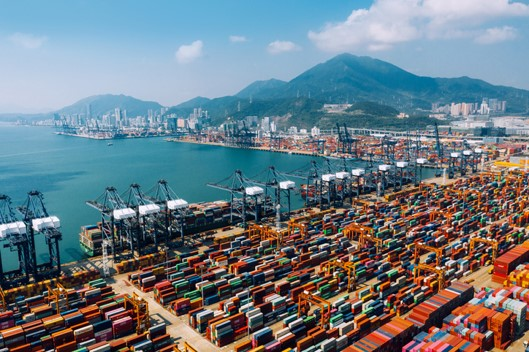
\includegraphics{./Images/Intro/Sea Port} 

}

\caption{Sea Port}(\#fig:Figure 2.11)
\end{figure}

Source: \url{https://www.porttechnology.org/news/what-are-sea-ports/\#}:\textasciitilde:text=Sea\%20ports\%20are\%20maritime\%20facilities,and\%20discharge\%20cargo\%20and\%20passengers.

\begin{enumerate}
\def\labelenumi{\arabic{enumi})}
\setcounter{enumi}{5}
\item
  The main functions of seaports are: To ensure safety for seagoing vessels entering, operation in and leaving the seaport. To provide facilities and equipment necessary for seagoing vessels to anchor, load and unload cargo, and embark and disembark passengers.
\item
  Ports are land facilities constructed to transfer goods between water and land. They consist of major features such as:
\end{enumerate}

\begin{enumerate}
\def\labelenumi{\alph{enumi})}
\tightlist
\item
  Docks or berths where vessels moor;
\item
  Equipment and personnel to load and unload vessels;
\item
  Connections to land transportation (such as highways, railways, and pipelines); and
\item
  Cargo storage areas.
\end{enumerate}

\hypertarget{intro-Tonnage_Port}{%
\section{Top 25 Tonnage Ports in 2020}\label{intro-Tonnage_Port}}

\begin{enumerate}
\def\labelenumi{\arabic{enumi})}
\item
  According to USDOT, Bureau of Transportation Statistics-The top 25 tonnage ports handled a total of 1,744 million tons of cargo about 71.3 percent of the tonnage handled by the top 100 ranked ports. The top 100 ports account for 95.5 percent of total tonnage handled by U.S. ports.
\item
  The highest tonnage figures are associated with ports that handle large quantities of both liquid bulk cargo (e.g., petroleum or chemicals) and dry bulk cargo (e.g., coal or grain), such as the ports of Houston, South Louisiana, and Corpus Christi.
\item
  The 2020 top tonnage port was the port of Houston.
\end{enumerate}

\hypertarget{intro-busiest_Port}{%
\section{The busiest container ports in the United States}\label{intro-busiest_Port}}

\begin{enumerate}
\def\labelenumi{\arabic{enumi})}
\tightlist
\item
  Some of the largest and most crucial container gateways of the world are in the United States. The following list of the busiest container ports in the US includes important box hubs, which contribute significantly to the country's economy, while they also allow container movement across the oceans, supporting and facilitating global trade.
\end{enumerate}

\begin{enumerate}
\def\labelenumi{\alph{enumi})}
\tightlist
\item
  Port of Los Angeles, California - More than 9.2 million TEU in 2020
\item
  Port of Long Beach, California - More than 8.1 million TEU in 2020
\item
  Port of New York and New Jersey, New York - More than 7.5 million TEU in 2020
\item
  Port of Savannah, Georgia - More than 4.6 million TEU in 2020
\item
  The Northwest Seaport Alliance (Seattle and Tacoma), Washington - More than 3.3 million TEU in 2020
\item
  Port Houston, Texas - More than 2.9 million TEU in 2020
\item
  Port of Virginia, Virginia - More than 2.8 million TEU in 2020
\item
  Port of Oakland, California - More than 2.4 million TEU in 2020
\item
  South Carolina Ports, South Carolina - More than 2.3 million TEU in 2020
\item
  Port Miami, Florida - More than 1 million TEU in 2020
\end{enumerate}

Source: \url{https://container-news.com/top-10-the-busiest-container-ports-in-the-united-states/}

\hypertarget{intro-Seaport_goods}{%
\section{Sea port goods movement}\label{intro-Seaport_goods}}

\begin{enumerate}
\def\labelenumi{\arabic{enumi})}
\item
  The Nation's ports handle the lion's share of U.S. international trade and transportation.
\item
  Following Figure shows the monthly U.S. international freight value transported by vessel. Between January 2021 and October 2021, the monthly U.S. international freight value transported by vessel increased by about \$31 billion (22.6 percent) from \$139 billion in January 2021 to \$170 billion in October 2021 billion in October 2021.
\end{enumerate}

\begin{figure}

{\centering 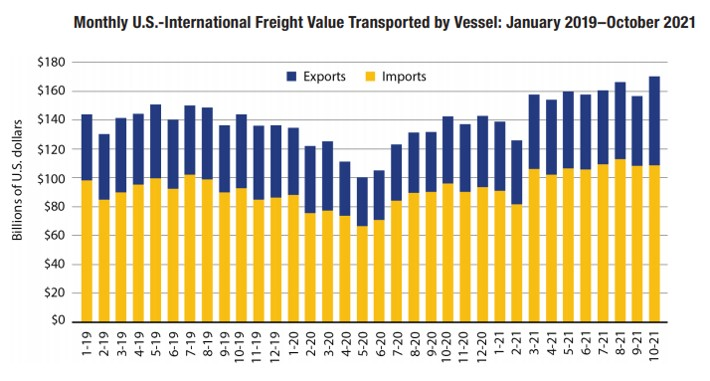
\includegraphics{./Images/Intro/Monthly U.S. international freight value} 

}

\caption{Monthly U.S. international freight value}(\#fig:Figure 2.12)
\end{figure}

Source: U.S. Department of Transportation, Bureau of Transportation Statistics analysis, based upon U.S. Department of Commerce, Census Bureau, USA Trade Online, available at \url{https://usatrade.census.gov/} as of December 2021.

\hypertarget{intro-container_port}{%
\section{Container Sea Ports}\label{intro-container_port}}

The operations of container seaport include four steps:

\begin{enumerate}
\def\labelenumi{\arabic{enumi})}
\tightlist
\item
  Ship-to-shore: stage when cargo is discharged
\item
  Transfer: cargo is unloaded to a temporal area
\item
  Storage: stage where containers are hold for a longer period of time
\item
  Delivery and receipt is the movement of delivery (clearance) of the cargo or receiving into the terminal
\end{enumerate}

\begin{figure}

{\centering 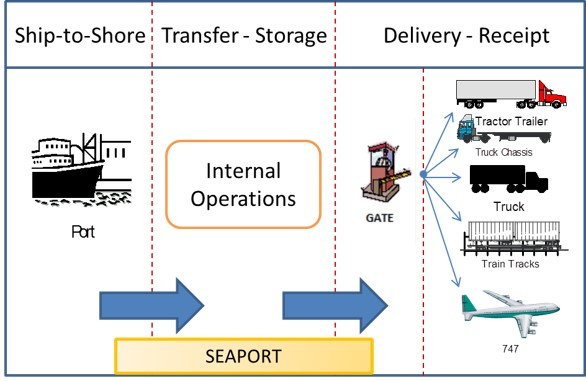
\includegraphics{./Images/Intro/Operations of container seaport} 

}

\caption{Operations of container seaport}(\#fig:Figure 2.13)
\end{figure}

\hypertarget{intro-container_terminal_structure}{%
\section{Container Terminal Structure}\label{intro-container_terminal_structure}}

A sea container terminal consists of at least three operational areas:

\begin{enumerate}
\def\labelenumi{\arabic{enumi})}
\item
  The operational area between the quay wall and container yard (area just behind the berth front).
\item
  The container yard (terminal storage, which is the stacking area): the area where the containers are stocked and where the loading and unloading activities of these units are carried out.
\item
  The terminal area of landside operations, which includes the gate, parking, office buildings, customs facilities, container freight station with an area for stuffing and stripping, empty container storage, a container maintenance and repair area, and so on.
\end{enumerate}

\begin{figure}

{\centering 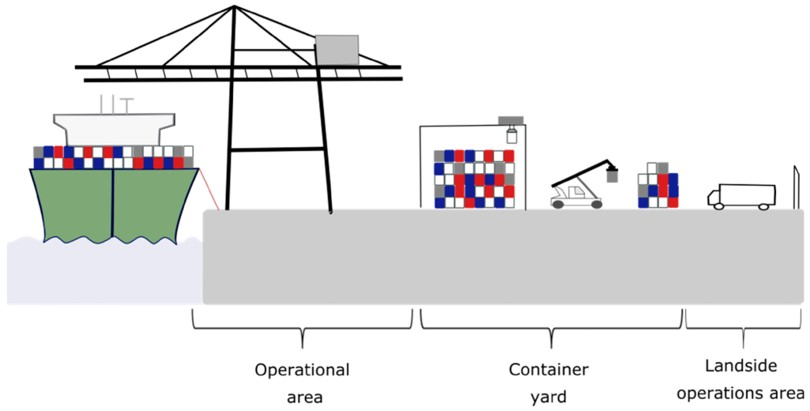
\includegraphics{./Images/Intro/Scheme of a port terminal of containers showing the three main zones} 

}

\caption{Scheme of a port terminal of containers showing the three main zones}(\#fig:Figure 2.14)
\end{figure}

\hypertarget{intro-Goods_movement}{%
\section{Goods movement in Seaport}\label{intro-Goods_movement}}

\begin{enumerate}
\def\labelenumi{\arabic{enumi})}
\item
  Let's assume a renowned Denim brand from the US wants to outsource its jeans consignment from China. Once the consignment is ready, the exporter will first select a particular shipping company whose container will come to its factory for cargo loading.
\item
  After loading the containers, the containers are sealed and an identical no. or a particular id is given to the exporter so that they can track their goods.
\item
  Now the Freight forwarder will arrange for the intermodal transport i.e.~transporting the container from the exporter warehouse or factory to the designated shipping port for loading into the ships.
\end{enumerate}

Shipping:

\begin{enumerate}
\def\labelenumi{\arabic{enumi})}
\item
  In the port, the container weights are measured, and the entries are made according to that. The container is stacked in the port in such a manner that they can be taken out easily as per the schedule of their assigned vessel. Now the container is ready to be loaded on the ship.
\item
  Once the ship arrives, the container is brought from the port storage facility, near to the ship by container port trucks
\item
  The container can be stored on the ship's cargo hold, where container guides are provided to draw and place the container inside the hold.
\item
  Once the ship reaches the destined port, the container will be unloaded by the port cranes, and it is transported to the port bay or warehouse using the port container trucks.
\item
  Once the custody of the shipment is acquired by the Importer's representative or by the freight forwarder, the cargo will be transported using intermodal transport to the importer's warehouse where the container is unloaded.
\item
  The empty container is now returned to the shipping line designated container yard, where it will wait for the next booking and onward journey.
\item
  The world is now connected by thousands of containers making it feasible for businesses and people to trade across the globe.
\end{enumerate}

\begin{figure}

{\centering 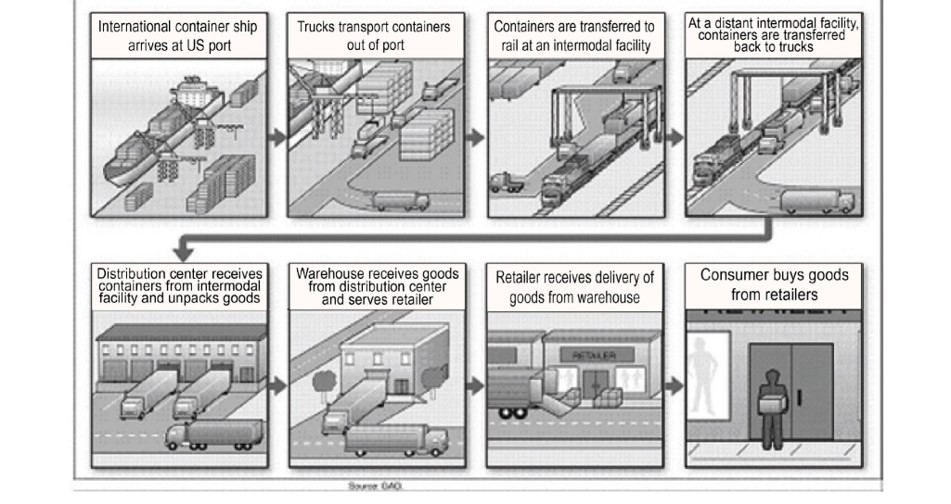
\includegraphics{./Images/Intro/Example of Goods movement from port of entry to customer} 

}

\caption{Example of Goods movement from port of entry to customer}(\#fig:Figure 2.15)
\end{figure}

\hypertarget{intro-port_Logistic}{%
\section{Sea-port Logistic}\label{intro-port_Logistic}}

For accessibility reasons, port-centric activities tend to cluster in areas close to or adjacent to port terminals. A better organization of first and second-tier activities is commonly leading to the setting of port-centric logistics zones. These zones have several advantages, including a better utilization level of transportation and container assets.

\begin{figure}

{\centering 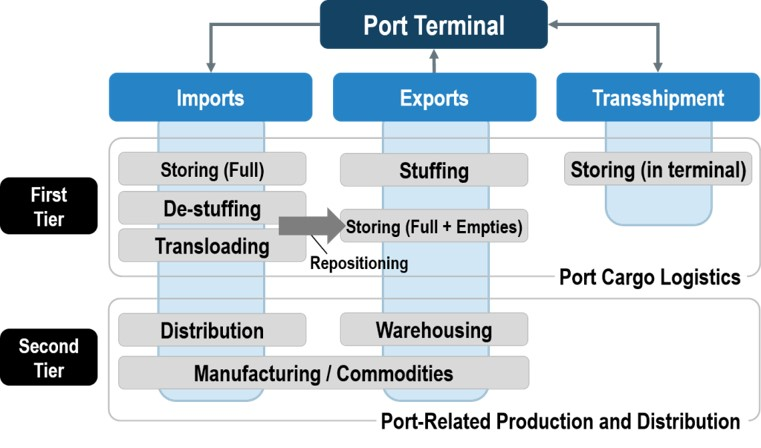
\includegraphics{./Images/Intro/Sea-port logistics} 

}

\caption{Sea-port logistics}(\#fig:Figure 2.16)
\end{figure}

\begin{figure}

{\centering 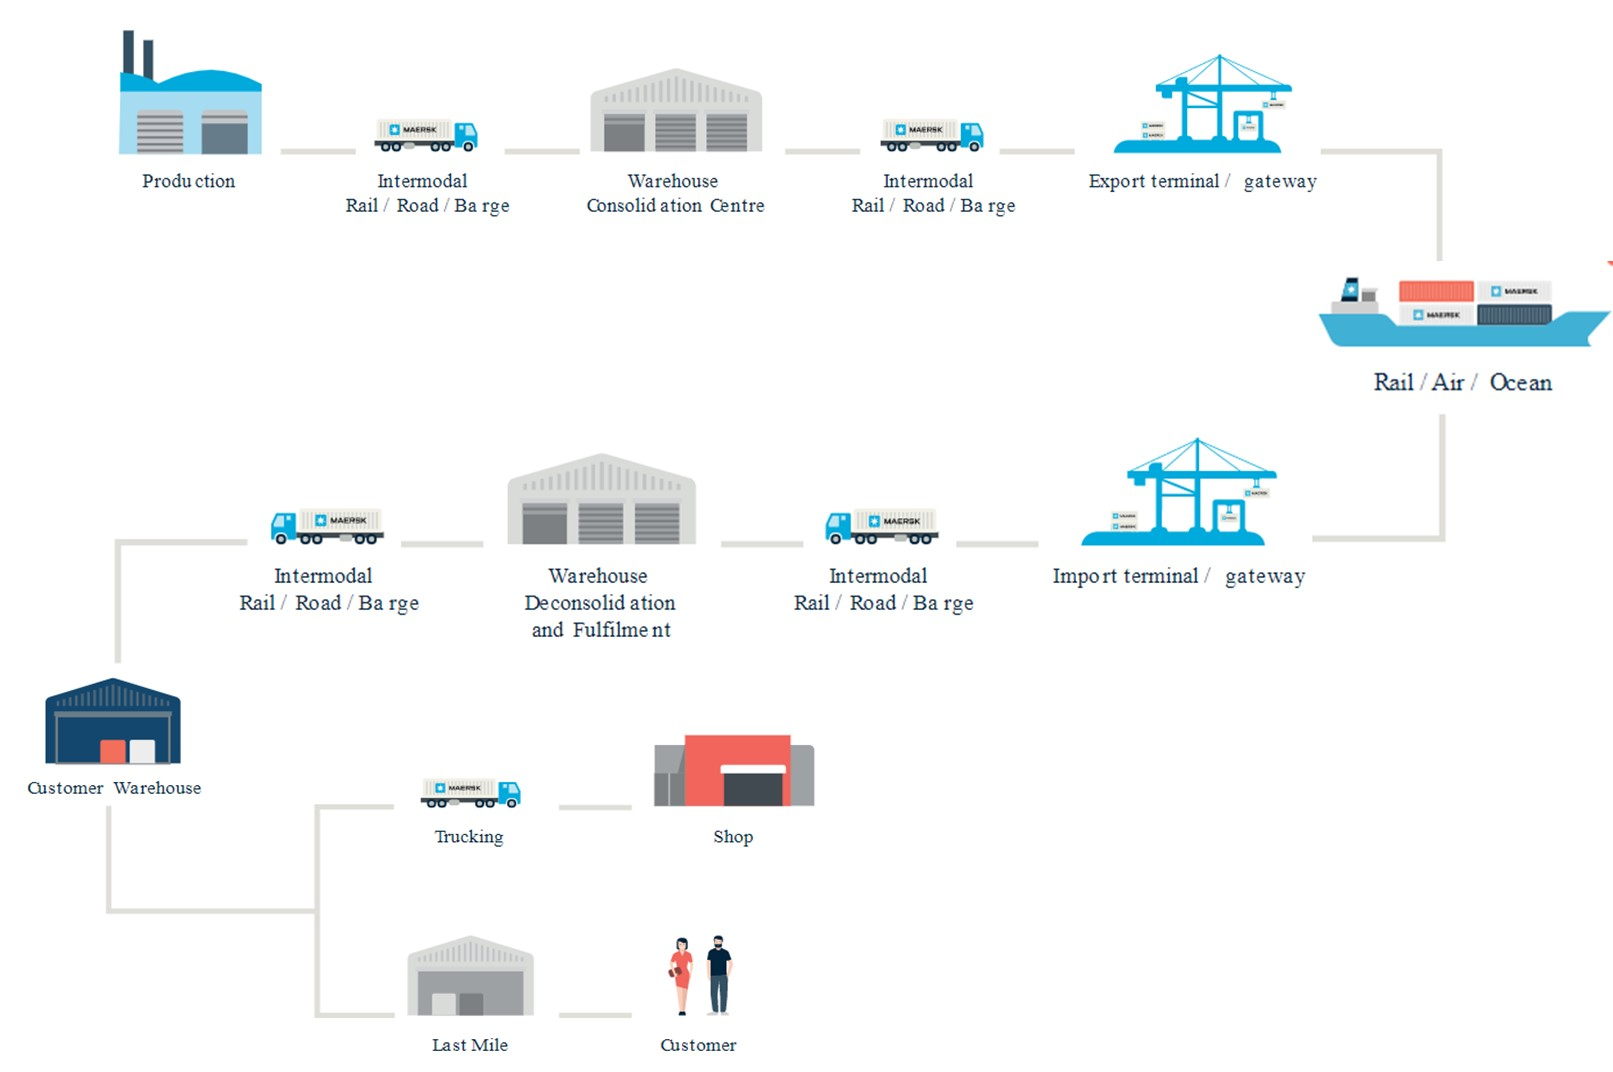
\includegraphics{./Images/Intro/Warehousing services} 

}

\caption{Warehousing services}(\#fig:Figure 2.17)
\end{figure}

\hypertarget{VehChars}{%
\chapter{Freight Vehicle Characteristics}\label{VehChars}}

\hypertarget{VehChars-Classes}{%
\section{FHWA truck classifications}\label{VehChars-Classes}}

\begin{figure}

{\centering 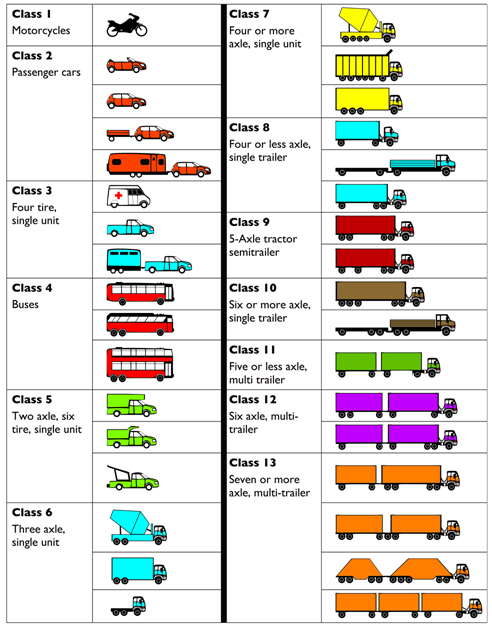
\includegraphics{./Images/VehClassesFHWA} 

}

\caption{FHWA truck Classifications}(\#fig:Figure 3.1)
\end{figure}

Source: FHWA (2019). Traffic Monitoring Guide, Appendix C. Vehicle Types. USDOT. Washington, DC. URL: \url{https://www.fhwa.dot.gov/policyinformation/tmguide/tmg_2013/vehicle-types.cfm}.

\hypertarget{types-of-trailers}{%
\section{Types of trailers}\label{types-of-trailers}}

\begin{enumerate}
\def\labelenumi{\arabic{enumi}.}
\tightlist
\item
  Flatbed Trailer
\item
  Dry Vans
\item
  Refrigerated Trailer
\item
  Lowboy Trailers
\item
  Step Deck Trailers
\item
  Etc.
\end{enumerate}

\url{https://truckfreighter.com/tractor-types-trucks-trailers}

An example table is shown in Table \ref{tab:Example}

\begin{longtable}[]{@{}cc@{}}
\caption{\label{tab:Example} A sample table}\tabularnewline
\toprule()
Variable & Value (\%) \\
\midrule()
\endfirsthead
\toprule()
Variable & Value (\%) \\
\midrule()
\endhead
X & 25 \\
Y & 50 \\
Z & 75 \\
\bottomrule()
\end{longtable}

\hypertarget{performance-characteristics-accel-decel-speed-governing-etc.}{%
\section{Performance characteristics (accel, decel, speed governing, etc.)}\label{performance-characteristics-accel-decel-speed-governing-etc.}}

\hypertarget{unloaded-weights}{%
\section{Unloaded weights}\label{unloaded-weights}}

\hypertarget{geometric-design-considerations-turning-radius-sight-distance-etc.}{%
\section{Geometric design considerations (turning radius, sight distance, etc.)}\label{geometric-design-considerations-turning-radius-sight-distance-etc.}}

\hypertarget{loading-characteristics}{%
\chapter{Loading Characteristics}\label{loading-characteristics}}

\hypertarget{maximum-load-without-permit-max-load-with-permit-route-restrictions-time-of-day-restrictions}{%
\section{Maximum load without permit, max load with permit, route restrictions, time of day restrictions}\label{maximum-load-without-permit-max-load-with-permit-route-restrictions-time-of-day-restrictions}}

\hypertarget{weigh-stations-weigh-in-motion}{%
\section{Weigh stations, weigh-in-motion}\label{weigh-stations-weigh-in-motion}}

\hypertarget{driver-issues}{%
\chapter{Driver issues}\label{driver-issues}}

\hypertarget{hours-of-service}{%
\section{Hours of service}\label{hours-of-service}}

\hypertarget{training}{%
\section{Training}\label{training}}

\hypertarget{recruitment}{%
\section{Recruitment}\label{recruitment}}

\hypertarget{parking}{%
\chapter{Parking}\label{parking}}

\hypertarget{parking-privateparking}{%
\section{private, such as Travel Centers of America/Petro}\label{parking-privateparking}}

Introduction:

Private parking advantages:

1.Important in urban areas where public parking is often limited.
Reduces congestion on road network.
2.Encourage the use of more sustainable forms of transportation, such as cycling and walking.
3.Provides convenient and reliable parking for users which improves users satisfaction and efficiency.

\begin{figure}

{\centering 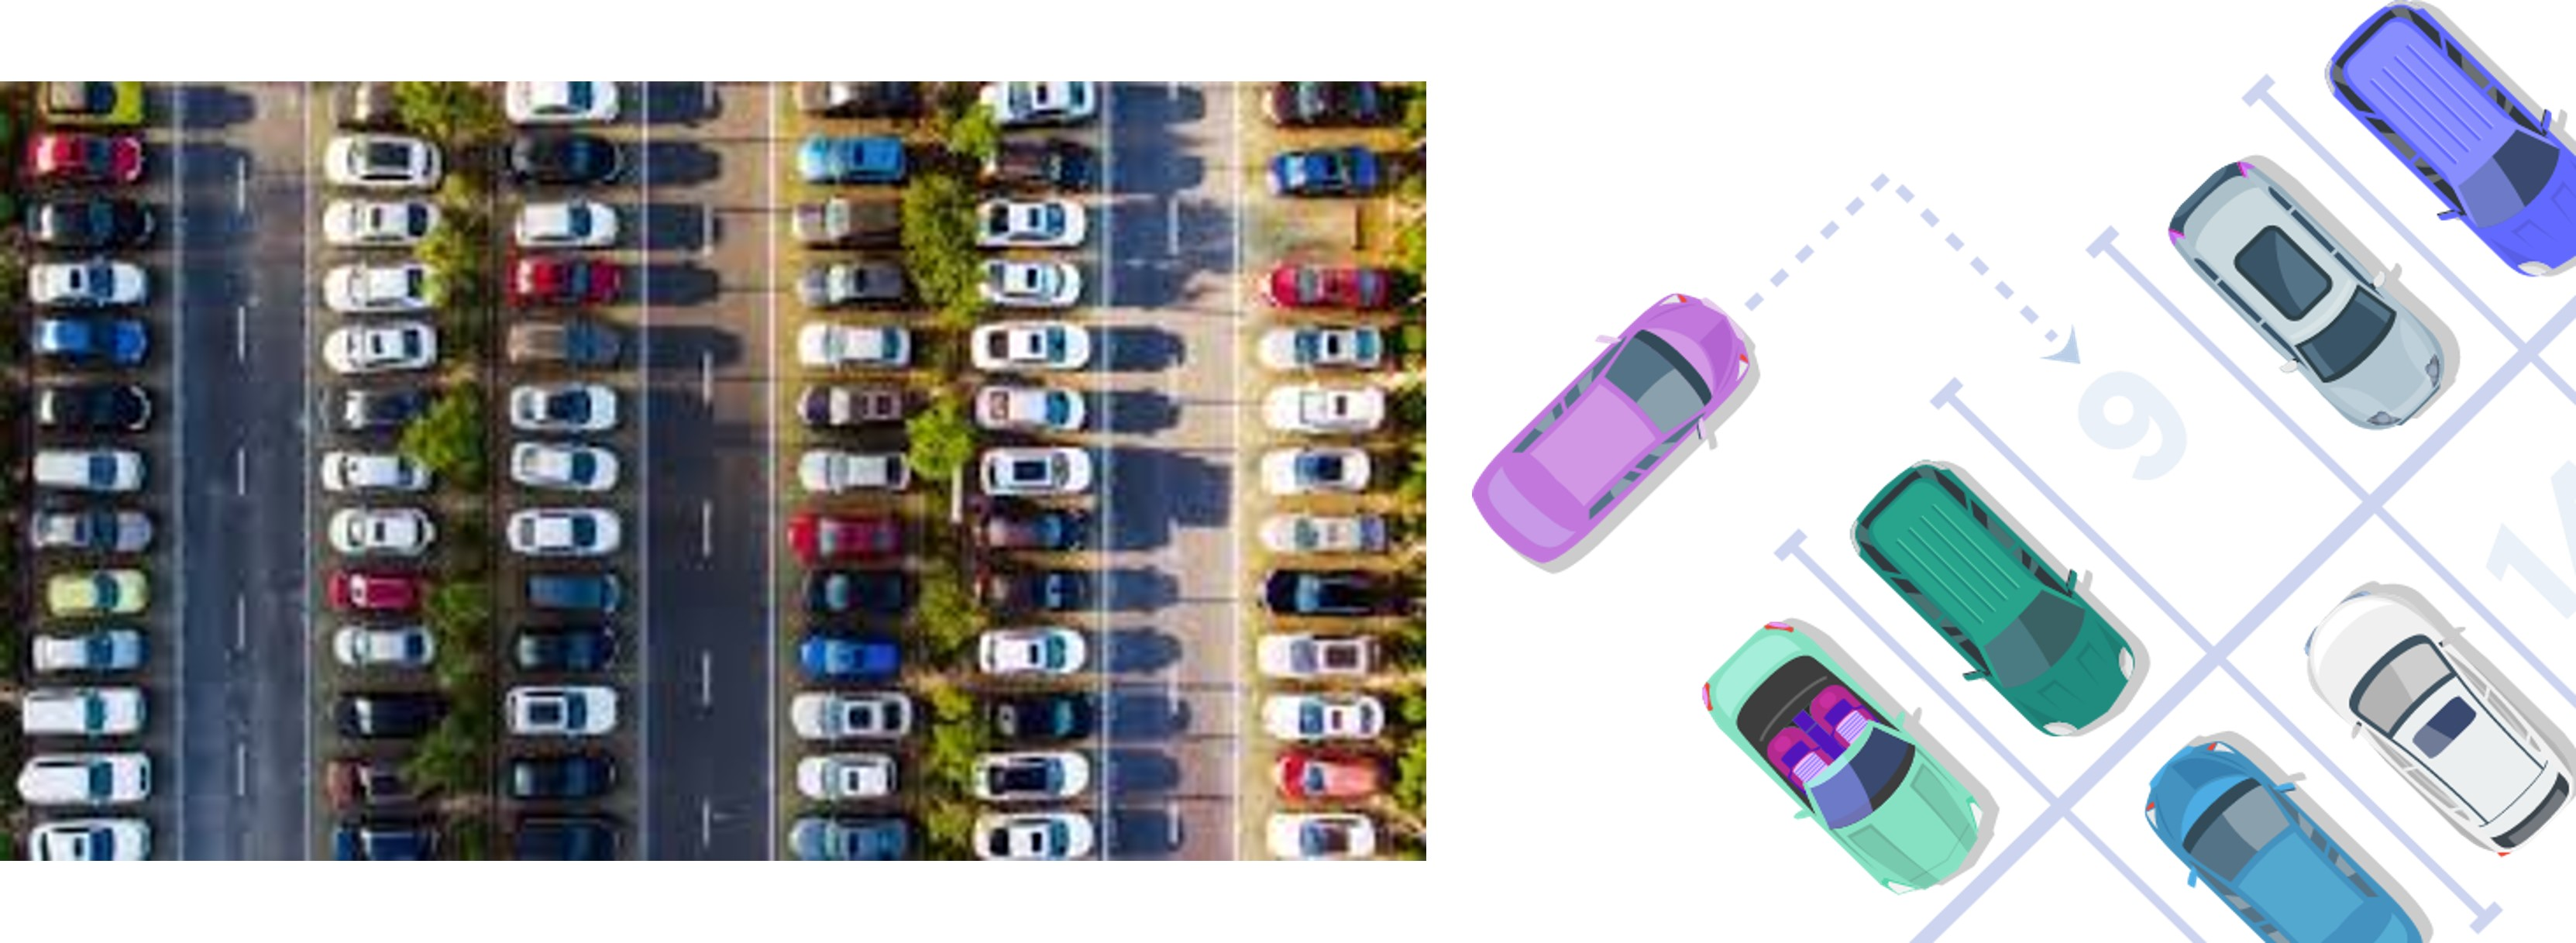
\includegraphics{./Images/Parking/Parking} 

}

\caption{Parking}(\#fig:Figure 6.1)
\end{figure}

4.Private parking can provide more accessibility and additional services but may come at a higher cost compared to alternative options which is typically more affordable but less available and may have fewer amenities.

\hypertarget{parking-benefits}{%
\section{Benefits of Private Parking}\label{parking-benefits}}

\begin{enumerate}
\def\labelenumi{\arabic{enumi}.}
\tightlist
\item
  Increased availability:
  Reducing competition
  Reserved for specific individuals or businesses
  Discouraging illegal parking
  Can reduce congestion and improve traffic flow.
  Encouraging carpooling:
  Groups of people can park in one private spot, freeing up public parking spots for others.
  Reducing circling time:
  Provide a designated space for vehicles. This can reduce traffic congestion and carbon emissions.
\end{enumerate}

\begin{figure}

{\centering 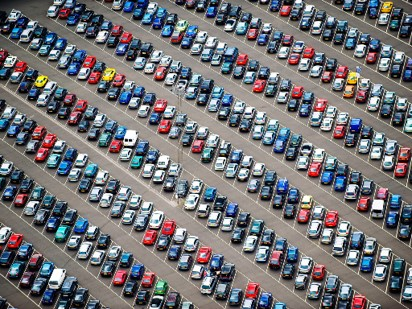
\includegraphics{./Images/Parking/Private Parking} 

}

\caption{Private Parking}(\#fig:Figure 6.2)
\end{figure}

\begin{enumerate}
\def\labelenumi{\arabic{enumi}.}
\setcounter{enumi}{1}
\tightlist
\item
  Convenience:
  Private parking facilities are often located in convenient locations:
  Shopping centers
  Tourist attractions
  Schools
  Airports
  Makes it easier for people to park their cars and access these areas on time.
\end{enumerate}

\begin{figure}

{\centering 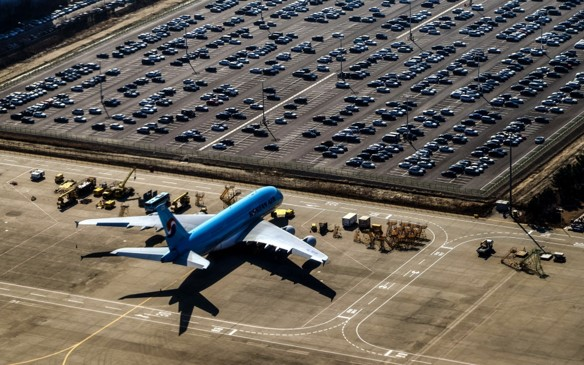
\includegraphics{./Images/Parking/Private Parking-Convenience} 

}

\caption{Private Parking-Convenience}(\#fig:Figure 6.3)
\end{figure}

\begin{enumerate}
\def\labelenumi{\arabic{enumi}.}
\setcounter{enumi}{2}
\tightlist
\item
  Security:
  Controlled access
  Typically restricted to authorized personnel and/or customers.
  Surveillance
  Equipped with surveillance cameras or security guards.
  Maintenance
  Maintained more regularly, reducing the risk of injuries.
  Lighting
  Easier for drivers to see and navigate through the parking lot.
\end{enumerate}

\begin{figure}

{\centering 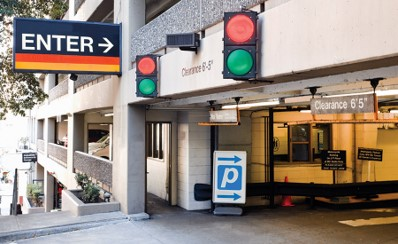
\includegraphics{./Images/Parking/Private Parking-Security} 

}

\caption{Private Parking-Security}(\#fig:Figure 6.4)
\end{figure}

\begin{enumerate}
\def\labelenumi{\arabic{enumi}.}
\setcounter{enumi}{3}
\tightlist
\item
  Cost-effectiveness:
  Competitive pricing
  Competitive pricing between facilities.
  Long-term contracts
  Provide discounts for customers who commit to a certain length of time.
  Reduced fees
  For frequent customers or for those who use their services during off-peak hours.
  May have reduced or waived fees for certain groups, such as disabled individuals or electric vehicle owners.
  Gives incentives towards users
\end{enumerate}

\begin{figure}

{\centering 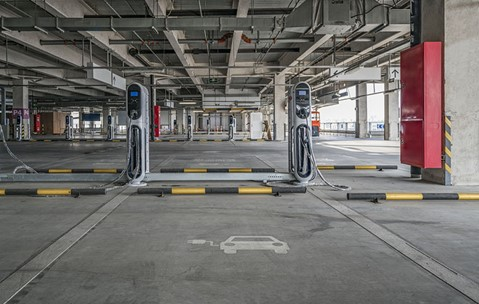
\includegraphics{./Images/Parking/Private Parking-Cost Effectiveness} 

}

\caption{Private Parking-Cost Effectiveness}(\#fig:Figure 6.5)
\end{figure}

\begin{enumerate}
\def\labelenumi{\arabic{enumi}.}
\setcounter{enumi}{4}
\tightlist
\item
  Technology:
  Online booking
  Saves time and ensure availability.
  Automated payment systems
  Such as pay-by-phone or contactless payment, making payment easier and more convenient for customers.
  License plate recognition
  Allows for automated entry and exit of vehicles.
  Parking guidance systems
  Help drivers locate available parking spots more easily.
\end{enumerate}

\begin{figure}

{\centering 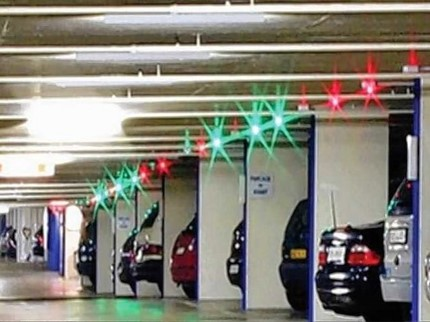
\includegraphics{./Images/Parking/Private Parking-Technology} 

}

\caption{Private Parking-Technology}(\#fig:Figure 6.6)
\end{figure}

\hypertarget{parking-needs}{%
\section{Who Needs Private Parking}\label{parking-needs}}

\begin{enumerate}
\def\labelenumi{\arabic{enumi}.}
\tightlist
\item
  Residential
  Residents are less likely to park on the streets
  Reducing traffic congestion in the area
\end{enumerate}

Provides a secure place for residents to park
Reducing the risk of theft, vandalism, and accidents

Can increase the value of residential properties as it is a desirable feature for many homebuyers

Designed to make the most efficient use of space
Optimize the parking area

2.Businesses:
Customers are more likely to visit businesses with accessible parking
Efficient and fast parking increases business' foot traffic and sales

Provides an enhanced customer experience
Customers are more likely to return with convenient parking

Improved image and reputation
Helps businesses project a more professional and polished image
Seen as a perk or benefit for employees, improving morale and retention

3.Trucks/Freight
Provides a secure and safe place for trucks and freight during extended parking periods

Can be located close to major highways and/or transportation hubs
This can save time and reduce transportation costs

Facilities may offer maintenance services, such as fueling, weight stations, and repairs
Reduces downtime of vehicles

Facilities may offer electronic logging devices, weigh station bypasses, and compliance with Hours of Service regulations

4.Passenger Vehicles:
Provides a secure space for your vehicle, reducing the risk of theft and damage

Located in convenient locations. This can minimize cost, time and reduce carbon emissions

Private parking can protect transportation modes from environmental elements, such as sun, rain, snow, and hail, and natural disasters.

Provide maintenance services, such as car washes, oil changes, and tire rotations.

The private parking industry is active in many states, but some states have a more active industry than others.
States with large urban areas tend to have a higher demand for private parking, as public parking is often limited or expensive
Some examples of states with active private parking industries include:
California
New York
Illinois
Texas
Florida

\begin{figure}

{\centering 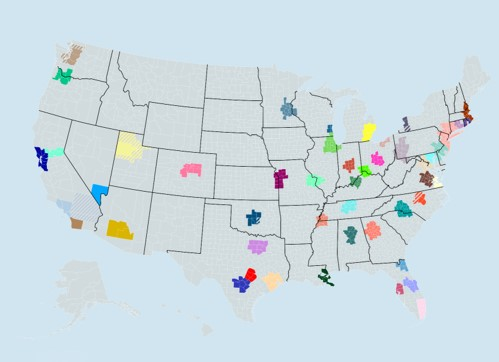
\includegraphics{./Images/Parking/Private Parking location} 

}

\caption{Private Parking location}(\#fig:Figure 6.7)
\end{figure}

\hypertarget{parking-companies}{%
\section{Private Parking Companies}\label{parking-companies}}

\begin{figure}

{\centering 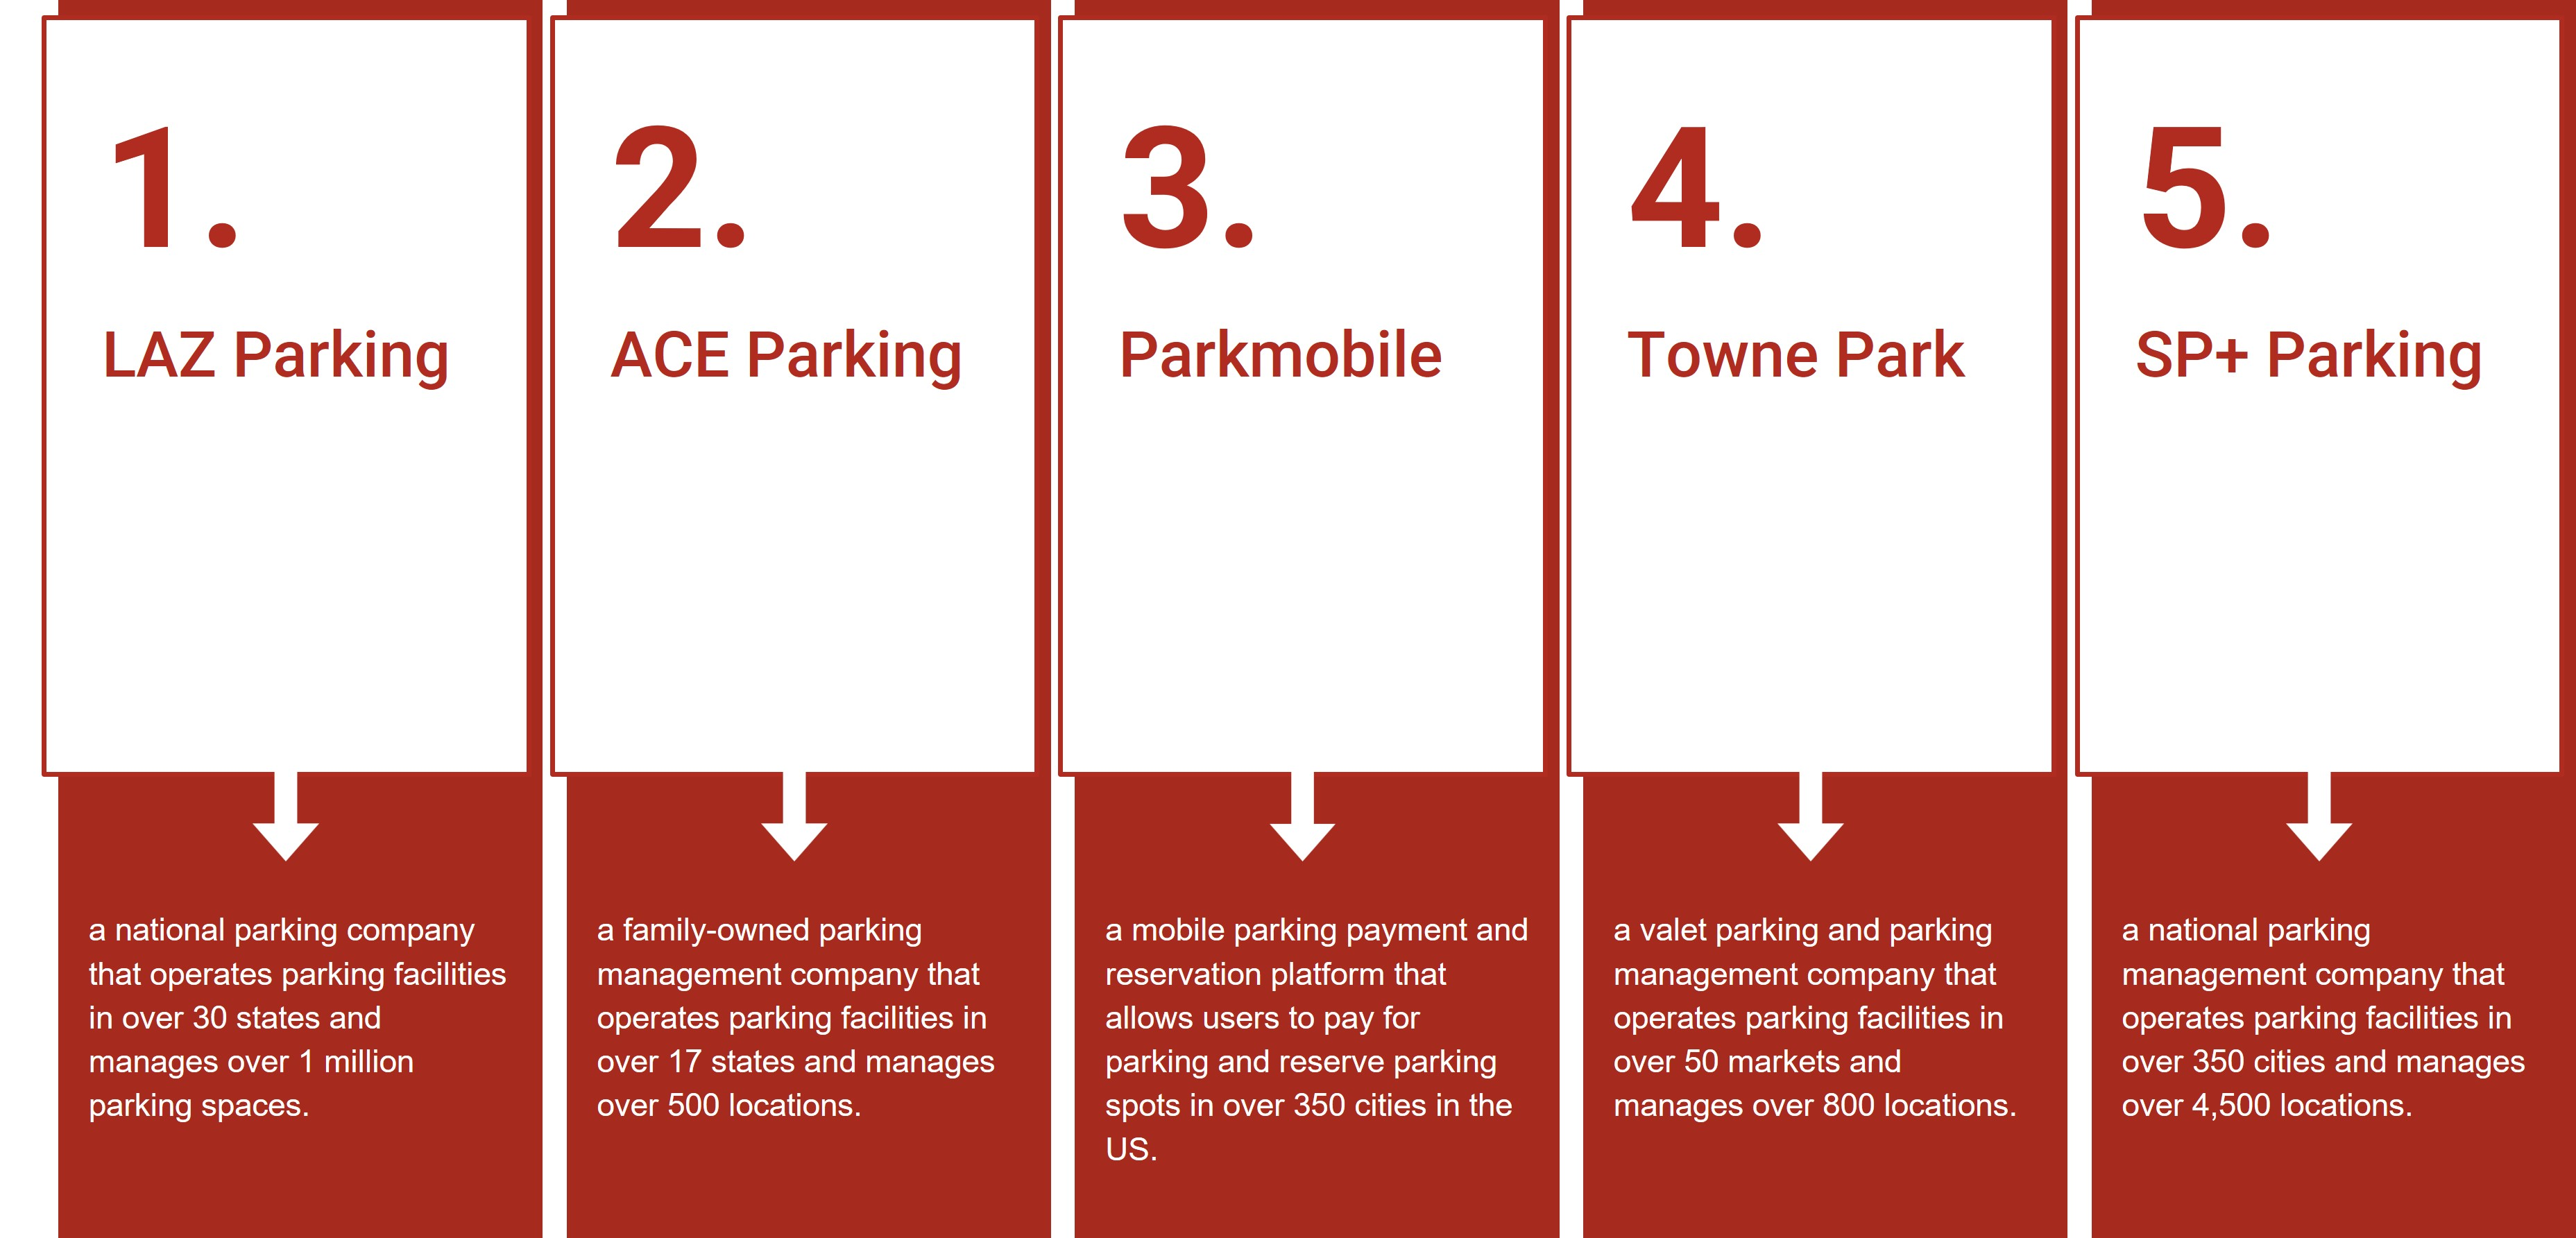
\includegraphics{./Images/Parking/Private Parking Companies} 

}

\caption{Private Parking Companies}(\#fig:Figure 6.8)
\end{figure}

\hypertarget{key-example-travelcenters-of-america-parking-travel-center}{%
\section{Key Example: TravelCenters of America \{\#parking-travel center\}}\label{key-example-travelcenters-of-america-parking-travel-center}}

TravelCenters of America (TA) is a chain of truck stops and travel centers primarily located in the U.S.

Served commercial drivers and highway travelers for over 50 years

Services offered:
Fuel stations, Restaurants, Convenience stores, Showers, Laundry facilities, Truck repair services.

Operates over 260 locations across the along major highways and interstates.

\begin{figure}

{\centering 
\includegraphics{./Images/Parking/Travel Centers of America} 

}

\caption{Travel Centers of America}(\#fig:Figure 6.9)
\end{figure}

\hypertarget{parking-conclusions}{%
\section{Conclusion}\label{parking-conclusions}}

Private parking can provide a range of benefits for drivers, businesses, and communities by providing:
A safer and efficient option for drivers
A cost-effective solution for individuals and/or businesses
Convenient, accommodating, and user-friendly technology
Applied mobile apps
Smart parking
Park guidance systems
Optimize time and provide efficiency in daily activities

\hypertarget{parking-availability-technologyinformation-systems}{%
\section{parking availability technology/information systems}\label{parking-availability-technologyinformation-systems}}

\hypertarget{SupplyChain}{%
\chapter{Supply Chain}\label{SupplyChain}}

\hypertarget{SupplyChain-Seaport}{%
\section{Sea Port}\label{SupplyChain-Seaport}}

Ports can serve a range of vessels including recreational watercraft, barges, ferries, and ocean-going cargo and passenger ships. The United States has over 150 deep-draft ports, which serve ocean-going ships.

Seaports are maritime facilities that can comprise one or more wharves where ships can dock to load and discharge cargo and passengers.

\hypertarget{SupplyChain-Seaportmng}{%
\section{Supply Chain Management}\label{SupplyChain-Seaportmng}}

Supply Chain Management (SCM) is the coordination and management of a complex network of activities delivering a finished product to end-users or customers.

The process includes sourcing raw materials and parts, manufacturing and assembling products, storage, order entry and tracking, distribution through the various channels, and finally delivery to the customer.

Seaports are functioning as platforms within global supply chains and global production networks.

These supply chains are highly dynamic as they react to changes in global trade patterns, consumer preferences, and advances in supply chain management and information technology.

\begin{figure}

{\centering 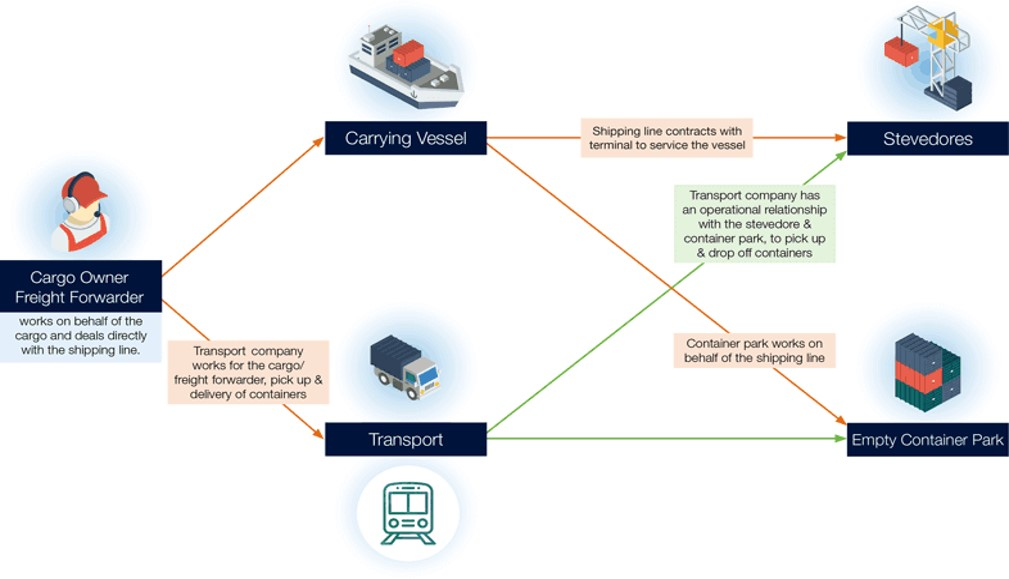
\includegraphics{./Images/supplychain/Ports and Supply Chain} 

}

\caption{Ports and Supply Chain}(\#fig:Figure 7.1)
\end{figure}

\hypertarget{SupplyChain-Seaportrole}{%
\section{The role of ports in the supply chain}\label{SupplyChain-Seaportrole}}

1.Ports are a nexus in supply chains as they support the interaction between global supply chains and regional production and consumption markets.

2.Global supply chains have become complex, pressuring the logistics industry to simultaneously improve their costs, performance, and resilience to disruptions.

3.Logistics services that still offer value may experience a debasement and become basic services, only generating a small margin. This is especially the case for physical added value.

4.The successful management of a supply chain is influenced by customer expectations, globalization, technological innovations, government regulation, competition, and sustainability concerns.

5.Within supply chains, corporations interact with external suppliers, internal departments, external distributors, and customers.

\begin{figure}

{\centering 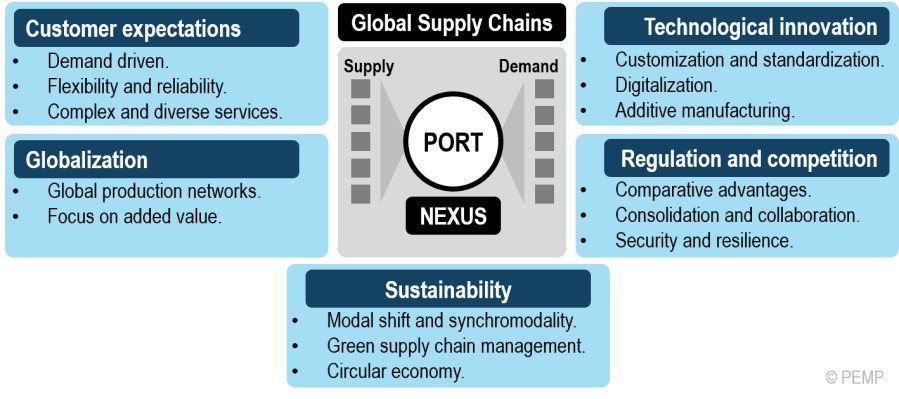
\includegraphics{./Images/supplychain/The role of ports in the supply chain} 

}

\caption{The role of ports in the supply chain}(\#fig:Figure 7.2)
\end{figure}

\hypertarget{ports-and-their-impact-on-the-global-supply-chain-supplychain-seaport-impact}{%
\section{Ports and Their Impact on the Global Supply Chain \{\#SupplyChain-Seaport impact\}}\label{ports-and-their-impact-on-the-global-supply-chain-supplychain-seaport-impact}}

\begin{enumerate}
\def\labelenumi{\arabic{enumi}.}
\tightlist
\item
  An efficient supply chain relies on optimized relationships, effective technology, excellent information sharing and streamlined infrastructure.
\item
  Port efficiency impacts organizations throughout the supply chain---suppliers, manufacturers, logistics service providers (LSPs), freight forwarders, cargo shipping lines and others.
\end{enumerate}

\begin{figure}

{\centering 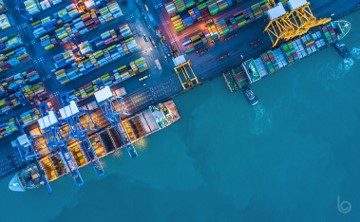
\includegraphics{./Images/supplychain/Ports and Their Impact on the Global Supply Chain} 

}

\caption{Ports and Their Impact on the Global Supply Chain}(\#fig:Figure 7.3)
\end{figure}

\begin{enumerate}
\def\labelenumi{\arabic{enumi}.}
\setcounter{enumi}{2}
\tightlist
\item
  Some of the problems with the current port system and discuss possible solutions to help streamline port and downstream supply chain operations:
\end{enumerate}

A Lack of Visibility into Container Status Impacts Forward Planning

A supply chain platform that integrates with port and terminal systems with a minimum of extra configuration
A centralized view of container status and information, so one can see where all your shipments are at a glance
Detailed container content information, so you can link specific supplies, parts and finished products back to loading, unloading and transportation schedules

\begin{enumerate}
\def\labelenumi{\arabic{enumi}.}
\setcounter{enumi}{3}
\tightlist
\item
  An Increase in Demand on Ports Can Make Carriers Less Efficient
\end{enumerate}

Deep analytics into exactly how ports are processing your shipments
Predictive forecasting and modeling so you can proactively make changes to your fleet operations
At-a-glance and in-depth reporting on the movement of goods so you can quickly identify and resolve potential issues

\begin{enumerate}
\def\labelenumi{\arabic{enumi}.}
\setcounter{enumi}{4}
\tightlist
\item
  Infrastructure and Transportation Within and Around a Port Makes a Big Difference
\end{enumerate}

Optimize routing and fleet transport through artificial intelligence, machine learning and predictive analytics
Accurate tracking of exactly where your containers, trucks, chassis and other assets are through GPS positioning
Take into account specialized handling needs for different types of sensitive goods

\begin{enumerate}
\def\labelenumi{\arabic{enumi}.}
\setcounter{enumi}{5}
\tightlist
\item
  Environmental Factors Can Impact on Ports and the Supply Chain
\end{enumerate}

The latest updates from air, ocean, rail and motor carriers
Communications from airport, marine and rail terminals
Data from electronic logging devices, automated information systems and GPS location services
Air traffic, weather alerts and maritime conditions

\begin{enumerate}
\def\labelenumi{\arabic{enumi}.}
\setcounter{enumi}{6}
\tightlist
\item
  Specialized Port Arrangements Can Take Advantage of a Centralized Supply Chain Platform
\end{enumerate}

\hypertarget{SupplyChain-Railport}{%
\section{Rail Ports}\label{SupplyChain-Railport}}

\hypertarget{SupplyChain-RailTransport}{%
\section{Rail Transport}\label{SupplyChain-RailTransport}}

1.Rail transport describes the usage of a train to transport passengers and freight along a designated route. Rail vehicles are directionally guided by the tracks on which they run and cannot deviate.

2.All across the globe, railroads are utilized to increase connectivity between regions and are major factors in developing countries.

\hypertarget{SupplyChain-Railroadnetwork}{%
\section{Railroad Network}\label{SupplyChain-Railroadnetwork}}

1.The United States freight rail network runs on almost 140,000 route miles. It is generally considered the largest, safest and most cost-effective means of transporting freight.

2.Unlike roadways, these freight railroads are owned and operated by private organizations such as CSX, BNSF and many others.

3.This railroad network is a series of different railroad classes that all work together to create a smooth shipment process.

\begin{figure}

{\centering 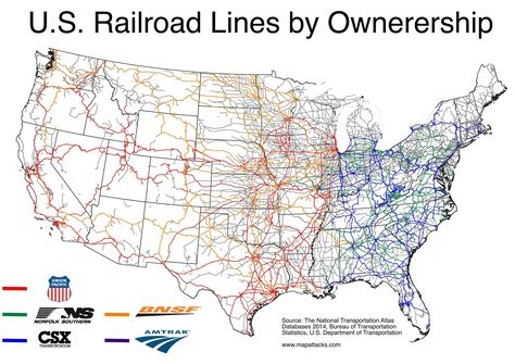
\includegraphics{./Images/supplychain/Railroad Network} 

}

\caption{Railroad Network}(\#fig:Figure 7.4)
\end{figure}

\begin{figure}

{\centering 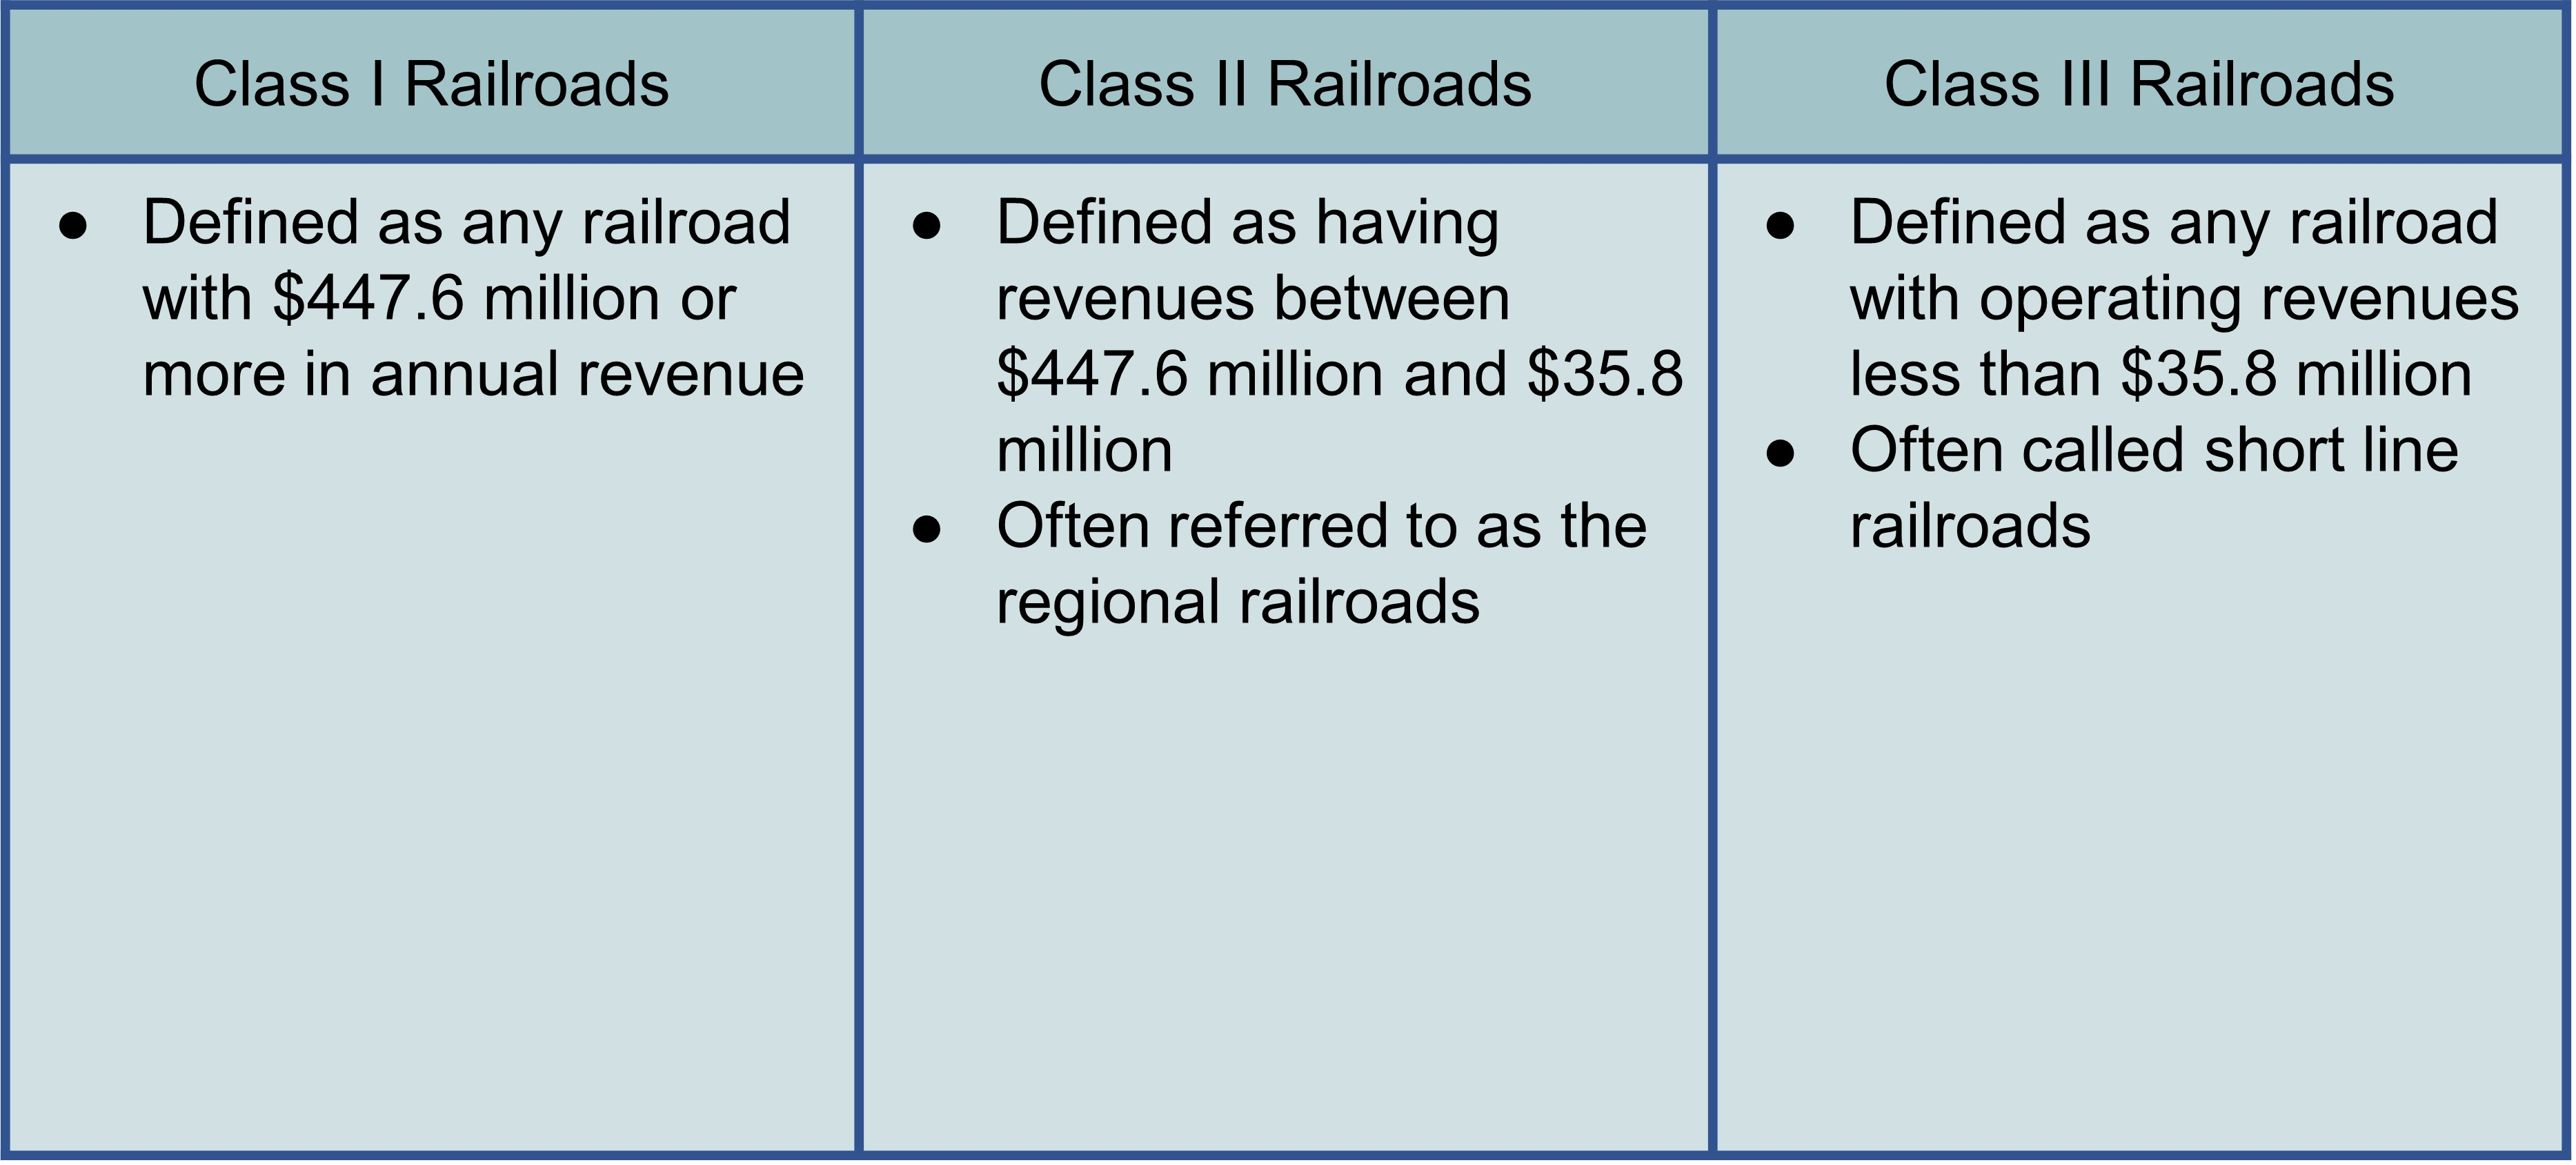
\includegraphics{./Images/supplychain/Types of Railroads} 

}

\caption{Types of Railroads}(\#fig:Figure 7.5)
\end{figure}

\hypertarget{SupplyChain-Railroad}{%
\section{How can freight railroads be accessed?}\label{SupplyChain-Railroad}}

\begin{enumerate}
\def\labelenumi{\arabic{enumi}.}
\item
  Along the main rail network, there are what are known as railroad sidings.
\item
  A railroad siding is a small stretch of track designed for minimal traffic and low speeds. These tracks are accompanied by warehouses to be used to store and transport goods from region to region.
\item
  Railroad sidings make distribution simpler by increasing the proximity of the warehouse to the route and decreasing overall transportation costs but are not always available to smaller manufacturers.
\end{enumerate}

\hypertarget{SupplyChain-whatisRailport}{%
\section{What is a Rail-port?}\label{SupplyChain-whatisRailport}}

1.Rail-ports are gateway centers which provide a multitude of services in addition to rail / road transshipment, warehousing and pre- and on-carriage by truck tailored to each customer's needs.

2.Rail-ports are a great alternative for companies than cannot afford their own warehouse and rail sidings. Rail-ports are ideal for handling bulk goods of all kinds- packed/loose, solid/pourable, palleted or in containers.

3.The Rail-port concept combines the benefits of rail, truck and regional warehouses.

\begin{figure}

{\centering 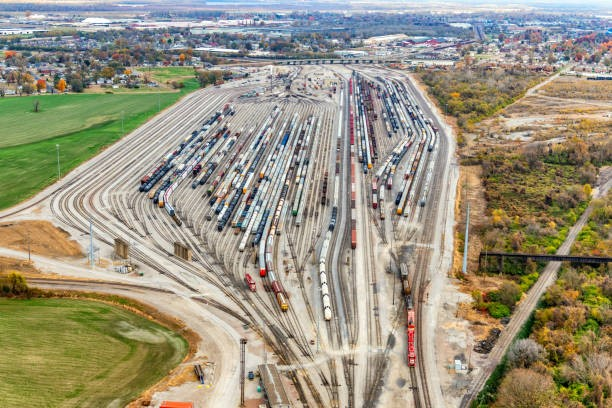
\includegraphics{./Images/supplychain/Rail-port} 

}

\caption{Rail-port}(\#fig:Figure 7.6)
\end{figure}

\hypertarget{SupplyChain-Railporttypes}{%
\section{Types of Rail Terminals}\label{SupplyChain-Railporttypes}}

1.Bulk
linked with extractive industries such as agriculture, mining,wood products, ect.
generally designed to be commodity specific.
2.Roll on/Roll off
Used to transport vehicles
require a large amount of parking space to store vehicles
3.Breakbulk
cargoes can be bagged, in drums, rolls or crates.
Containerization has reduced the need for breakbulk terminals
4.Intermodal
loading and unloading unitized freight from railcars
5.Shunting
assembly, sorting, and ``breaking'' of freight trains

\begin{figure}

{\centering 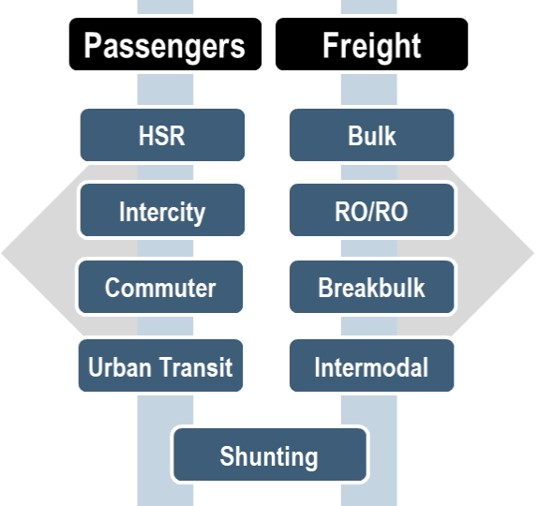
\includegraphics{./Images/supplychain/Types of Rail Terminals} 

}

\caption{Types of Rail Terminals}(\#fig:Figure 7.7)
\end{figure}

\#\#The Global Supply Chain \{\#SupplyChain-Railportglobal\}

Global freight supply chains are complex systems comprised of steamship lines, truckers, railroads, ports and a whole menagerie of other businesses and practices.

Railroads and Rail-ports function as an essential platforms within global supply chains and production networks.

These supply chains are ever evolving to keep up with changes in trade patterns, updated supply chain management and even new technologies.

\#\#The Role of Rail in the Supply Chain \{\#SupplyChain-Railportsupplychain\}
1. Railroads are considered the middleman of the supply chain. They move about 40\% of long-distance U.S. freight.

\begin{enumerate}
\def\labelenumi{\arabic{enumi}.}
\setcounter{enumi}{1}
\tightlist
\item
  They are an important conduit for freight between port and last-mile truck service. As such, freight has three transportation options upon arrival at a sea port:
\end{enumerate}

Off-dock: involves the movement of a container between the terminal and a railroad facility via truck over a distance
Near-dock: involves the movement of a container between the terminal adjacent but offsite railroad facility
On-dock: involves the direct loading of the container onto a train within the same terminal as the original vessel

\begin{figure}

{\centering 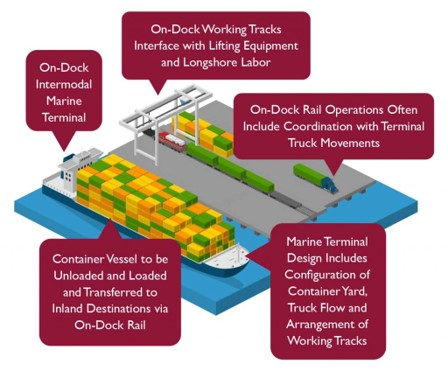
\includegraphics{./Images/supplychain/The Role of Rail in the Supply Chain} 

}

\caption{The Role of Rail in the Supply Chain}(\#fig:Figure 7.8)
\end{figure}

\begin{enumerate}
\def\labelenumi{\arabic{enumi}.}
\setcounter{enumi}{2}
\item
  Rail intermodal is the transportation method of moving freight across the globe by both railroad and truck.
\item
  As such, Intermodal provides both a competitively priced, and environmentally friendly alternative to excessive reliance on highways to transport freight.
\item
  Intermodal is focused on the 53' capacity freight market through the use of containers that move on the rail for the long haul segment of a shipment.There are two types of domestic intermodal shipping in container-on-flatcar (COFC) and trailer-on-flatcar.
\end{enumerate}

\begin{figure}

{\centering 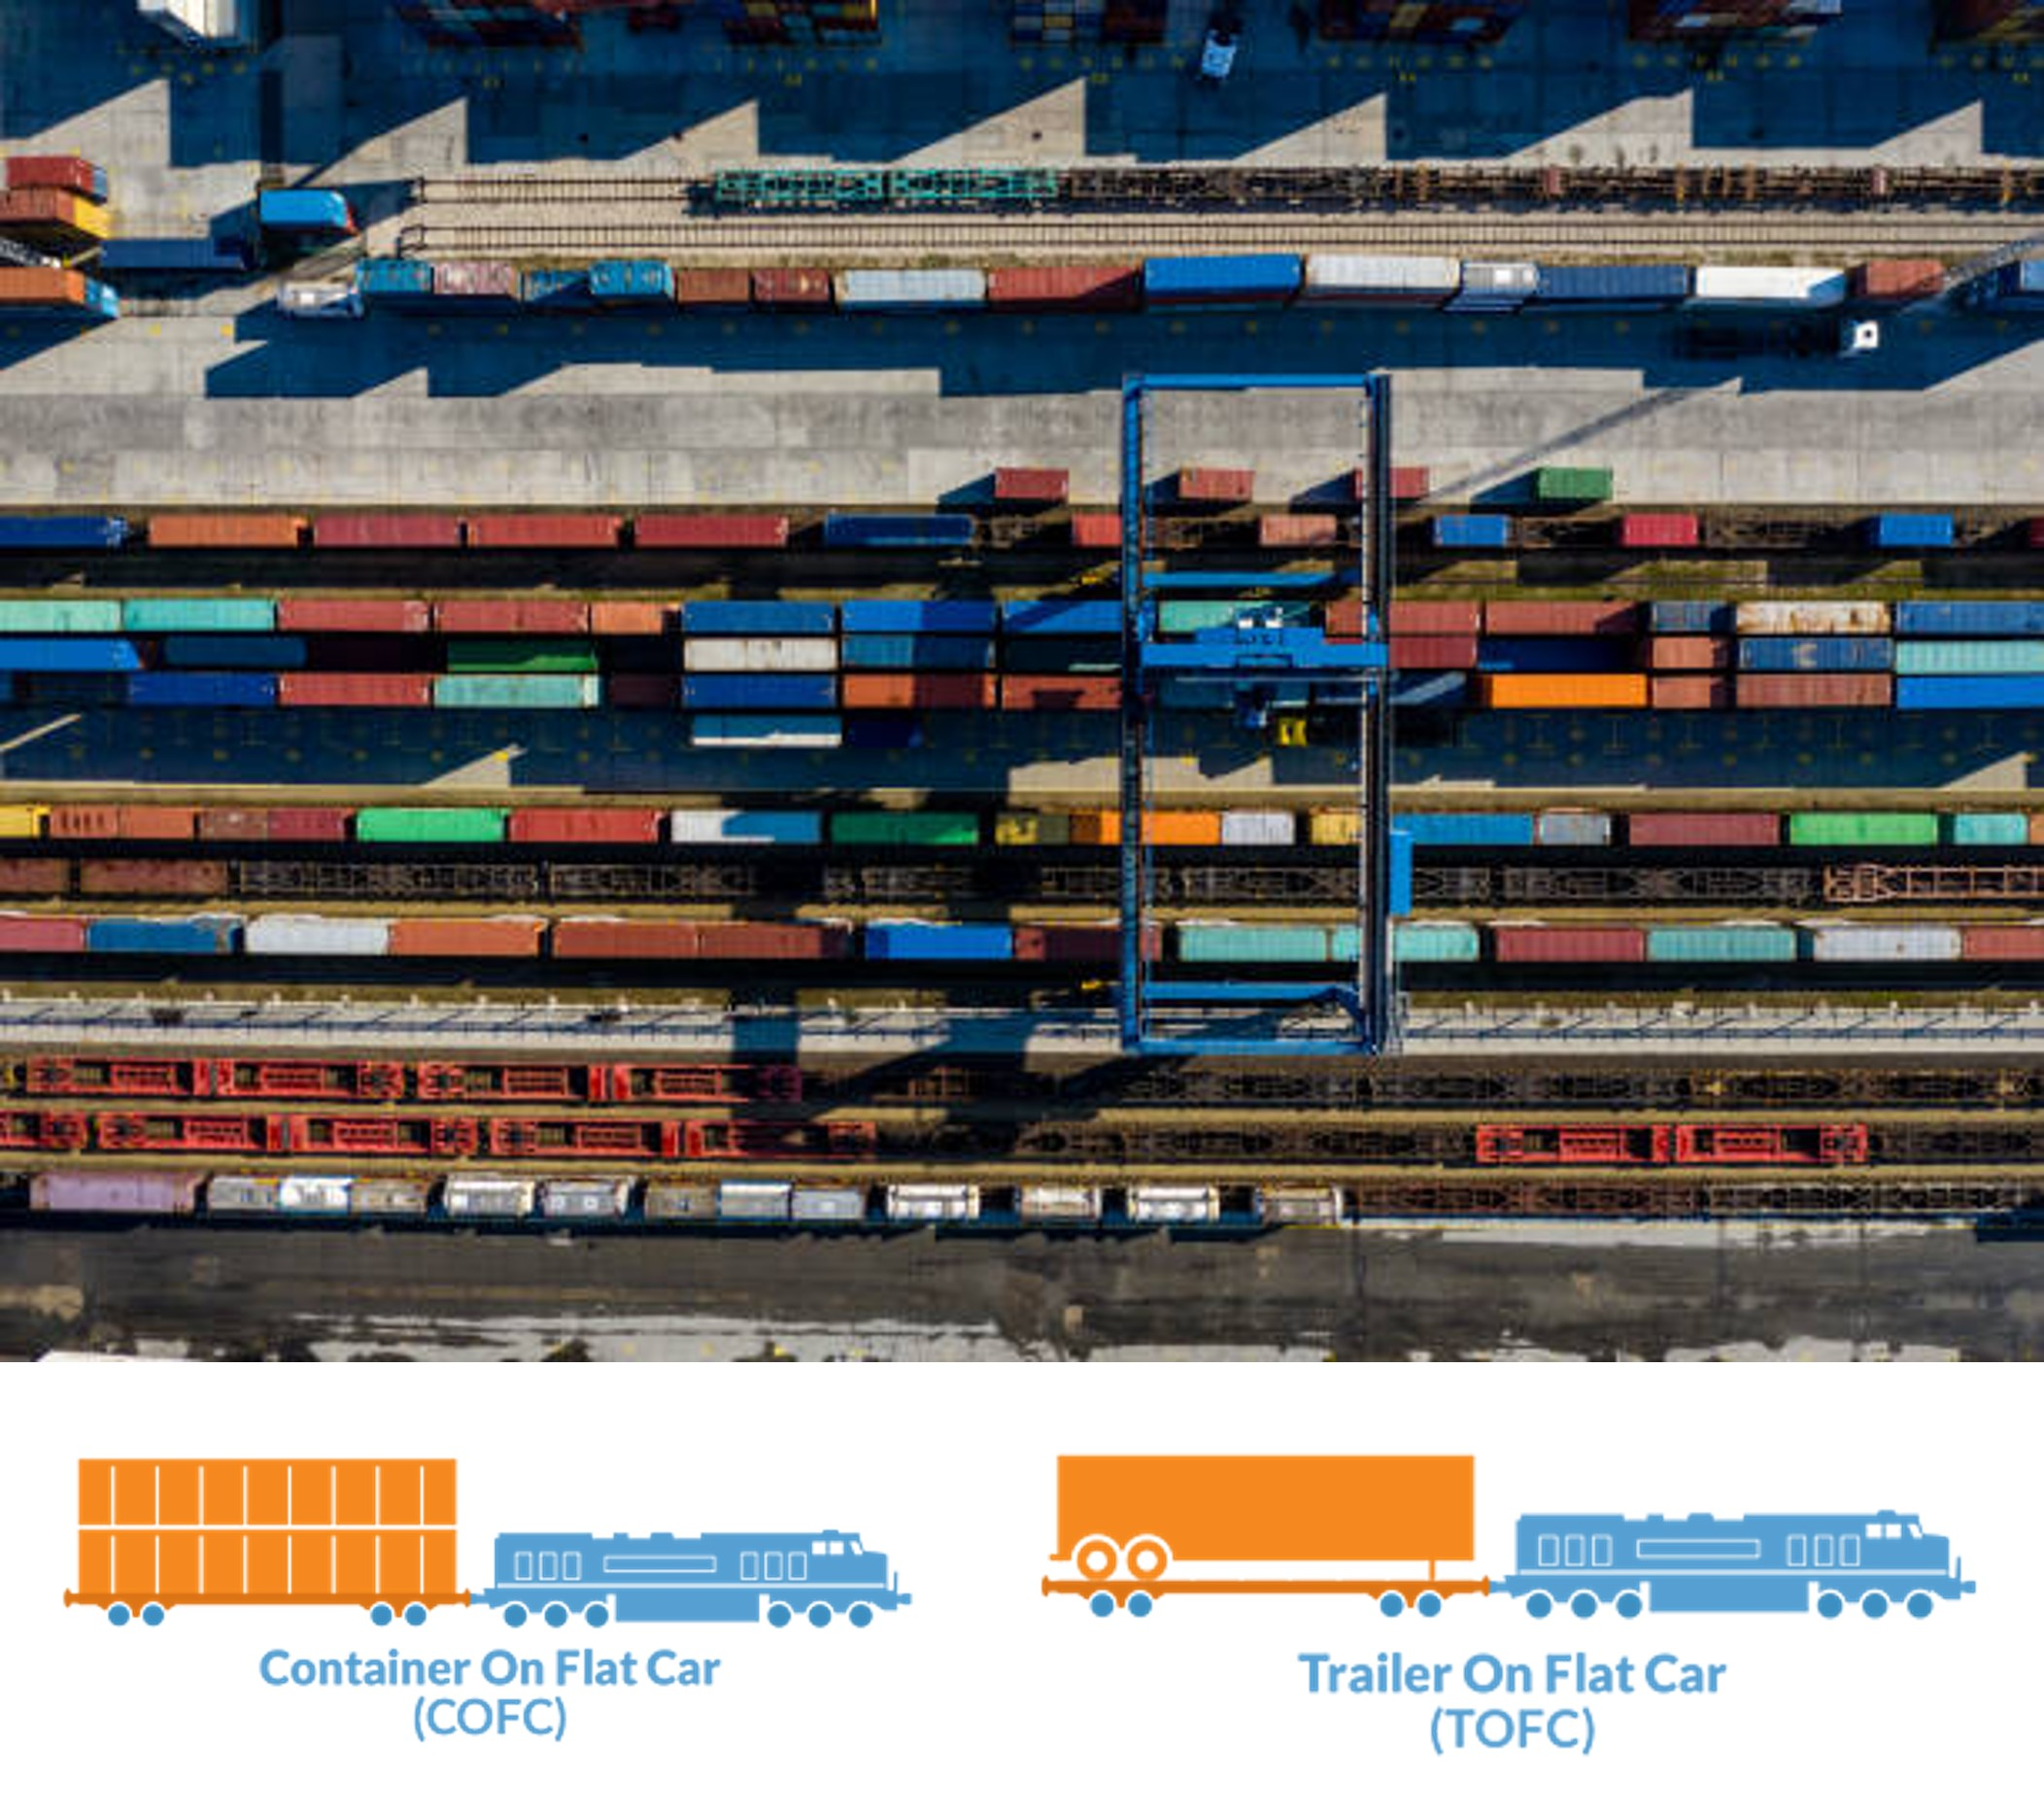
\includegraphics{./Images/supplychain/Role of Rail} 

}

\caption{Role of Rail}(\#fig:Figure 7.9)
\end{figure}

6.Per the Association of American Railroads:
Intermodal accounts for 25\% of the revenue for major U.S. railroads- more than any other traffic category
Half of the intermodal traffic is due to imports and exports

7.Aside from intermodal, railroads move commodities such as crude oil, ethanol and coal to help meet energy needs. It also moves essential chemicals such as fertilizers, plastic resins, caustic soda, and much more

\hypertarget{SupplyChain-Railportservice}{%
\section{Rail Service During Supply Chain Disruptions}\label{SupplyChain-Railportservice}}

1.In recent years the supply chain has been greatly impacted by the global pandemic by changes in on consumer purchasing trends, worker preferences, and rapidly changing global and national economies.

2.As the middle link in the supply network, rail service is impacted by these not only directly in how the other supply chain members interact with it.

\begin{figure}

{\centering 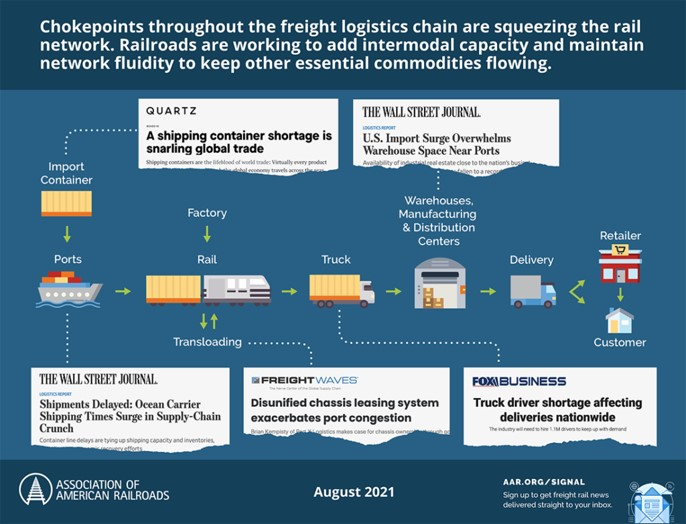
\includegraphics{./Images/supplychain/Rail Service During Supply Chain Disruptions} 

}

\caption{Rail Service During Supply Chain Disruptions}(\#fig:Figure 7.10)
\end{figure}

Rail networks have been combatting these disruptions by the following:

1.Expanding network capacity
Pulling equipment out of storage / activating their reserve fleets
Scheduling car movements to minimize congestion
Reopening of previously dormant terminals
2.Hiring, training, deploying and retaining train crews
Hiring bonuses, financial payments to refer-a-friend and other incentives to entice potential employees
Incentivizing through payments to move to high-demand regions of the network
Quick response to bring idled locomotives back online
3.Closely collaborating with trucks
Railroads and their trucking partners work to move shipments from intermodal terminals as quickly as possible\\
One railroad keeps a pool of truck chassis to help maximize truck hauling capacity while another railroad mounts intermodal containers on any chassis brought to it to help reduce truckers driving without any cargo

\hypertarget{SupplyChain-Railportimpact}{%
\section{The Economic Impact of Freight Railroads}\label{SupplyChain-Railportimpact}}

1.Freight railroads serve nearly every industrial, wholesale, retail and resource-based sector of the American economy.

2.The operations and capital investment of the freight rail industry has been estimated to support 1.1 percent of U.S. workers.

3.Railroads account for around 1/3 of U.S. exports by volume without which we would not be competitive in the global market.

\hypertarget{SupplyChain-FirstandLastMile}{%
\section{First/ Last Mile}\label{SupplyChain-FirstandLastMile}}

\hypertarget{SupplyChain-whatismile}{%
\section{What Is First/Last Mile?}\label{SupplyChain-whatismile}}

What is First Mile?
Depending on the Industry it can mean many things:
A manufacture may consider the First Mile when their completed goods are shipped from factory to their distribution hub.
A retailer may consider the First Mile when manufactured goods are shipped from suppliers' distribution hub to the retailer's distribution center.
E-commerce may consider the First Mile to be when the goods are transferred to the courier that will deliver the good to the costumer's home.
But in short, First Mile is when the good travels through the first leg of the supply chain.

\begin{figure}

{\centering 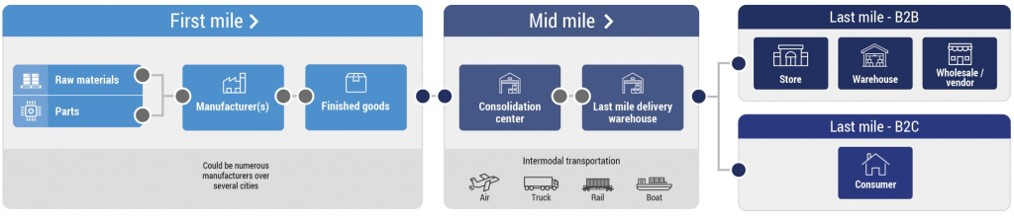
\includegraphics{./Images/supplychain/First and Last Mile} 

}

\caption{First and Last Mile}(\#fig:Figure 7.11)
\end{figure}

What is Last Mile?

Last Mile refers to the last phase of the supply chain process for the delivery of good or people.

Last Mile can be range anywhere from a couple of blocks to a couple 100 miles. The distance is determined by the network of the supply chain for the specific good being transported.

\begin{enumerate}
\def\labelenumi{\arabic{enumi}.}
\item
  Last Mile for Transporting Goods
  For transporting goods, the last
  mile may be the route taken by an Amazon driver to drop of packages.
  The route taken by an
  autonomous robot to deliver food.
\item
  Last Mile for Transporting People
  The last mile may be the taxi used to go
  from the airport to arrive at a hotel.
  The e-bike rental used to go from the
  train station to work (final destination).
\end{enumerate}

\begin{figure}

{\centering 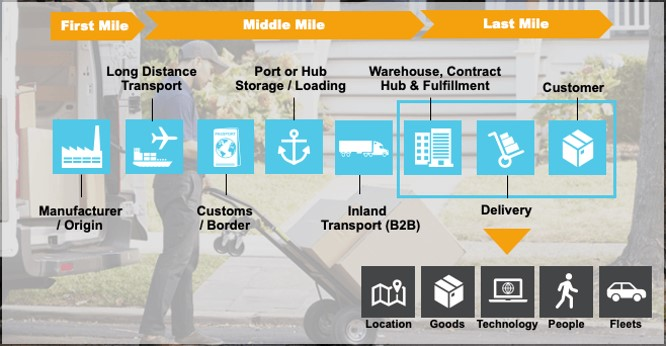
\includegraphics{./Images/supplychain/First and Last Mile Operation} 

}

\caption{First and Last Mile Operation}(\#fig:Figure 7.12)
\end{figure}

The concept of Last Mile was first introduced in the telecommunications industry.
The industry's Last Mile is the bandwidth that is delivered to the costumer.
The telecommunications network is like a ``tree''. Bandwidth that travels in high capacity are known as ``trunks''; the trunks branch out into ``twigs'' which serve as the Last Mile.

The Last Mile is a bandwidth bottleneck because there is a limit to how much data can be transferred to the costumer.
The Last Mile is also the most expensive because of all the equipment needed per customer and the number of customers that exist.

\begin{figure}

{\centering 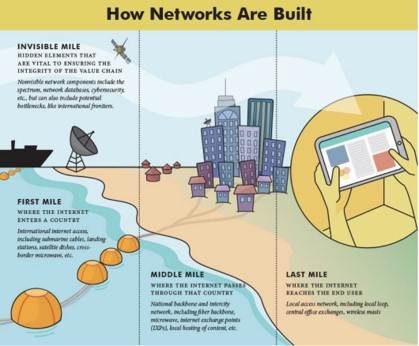
\includegraphics{./Images/supplychain/How Networks are Built} 

}

\caption{How Networks are Built}(\#fig:Figure 7.13)
\end{figure}

The concept of Last Mile first started with the telecommunications industry. But it has since branched out to other Industries. Most notably, the Transportation Industry

The remainder of this lecture will discuss First/Last Mile, and how it relates to transportation.

\begin{figure}

{\centering 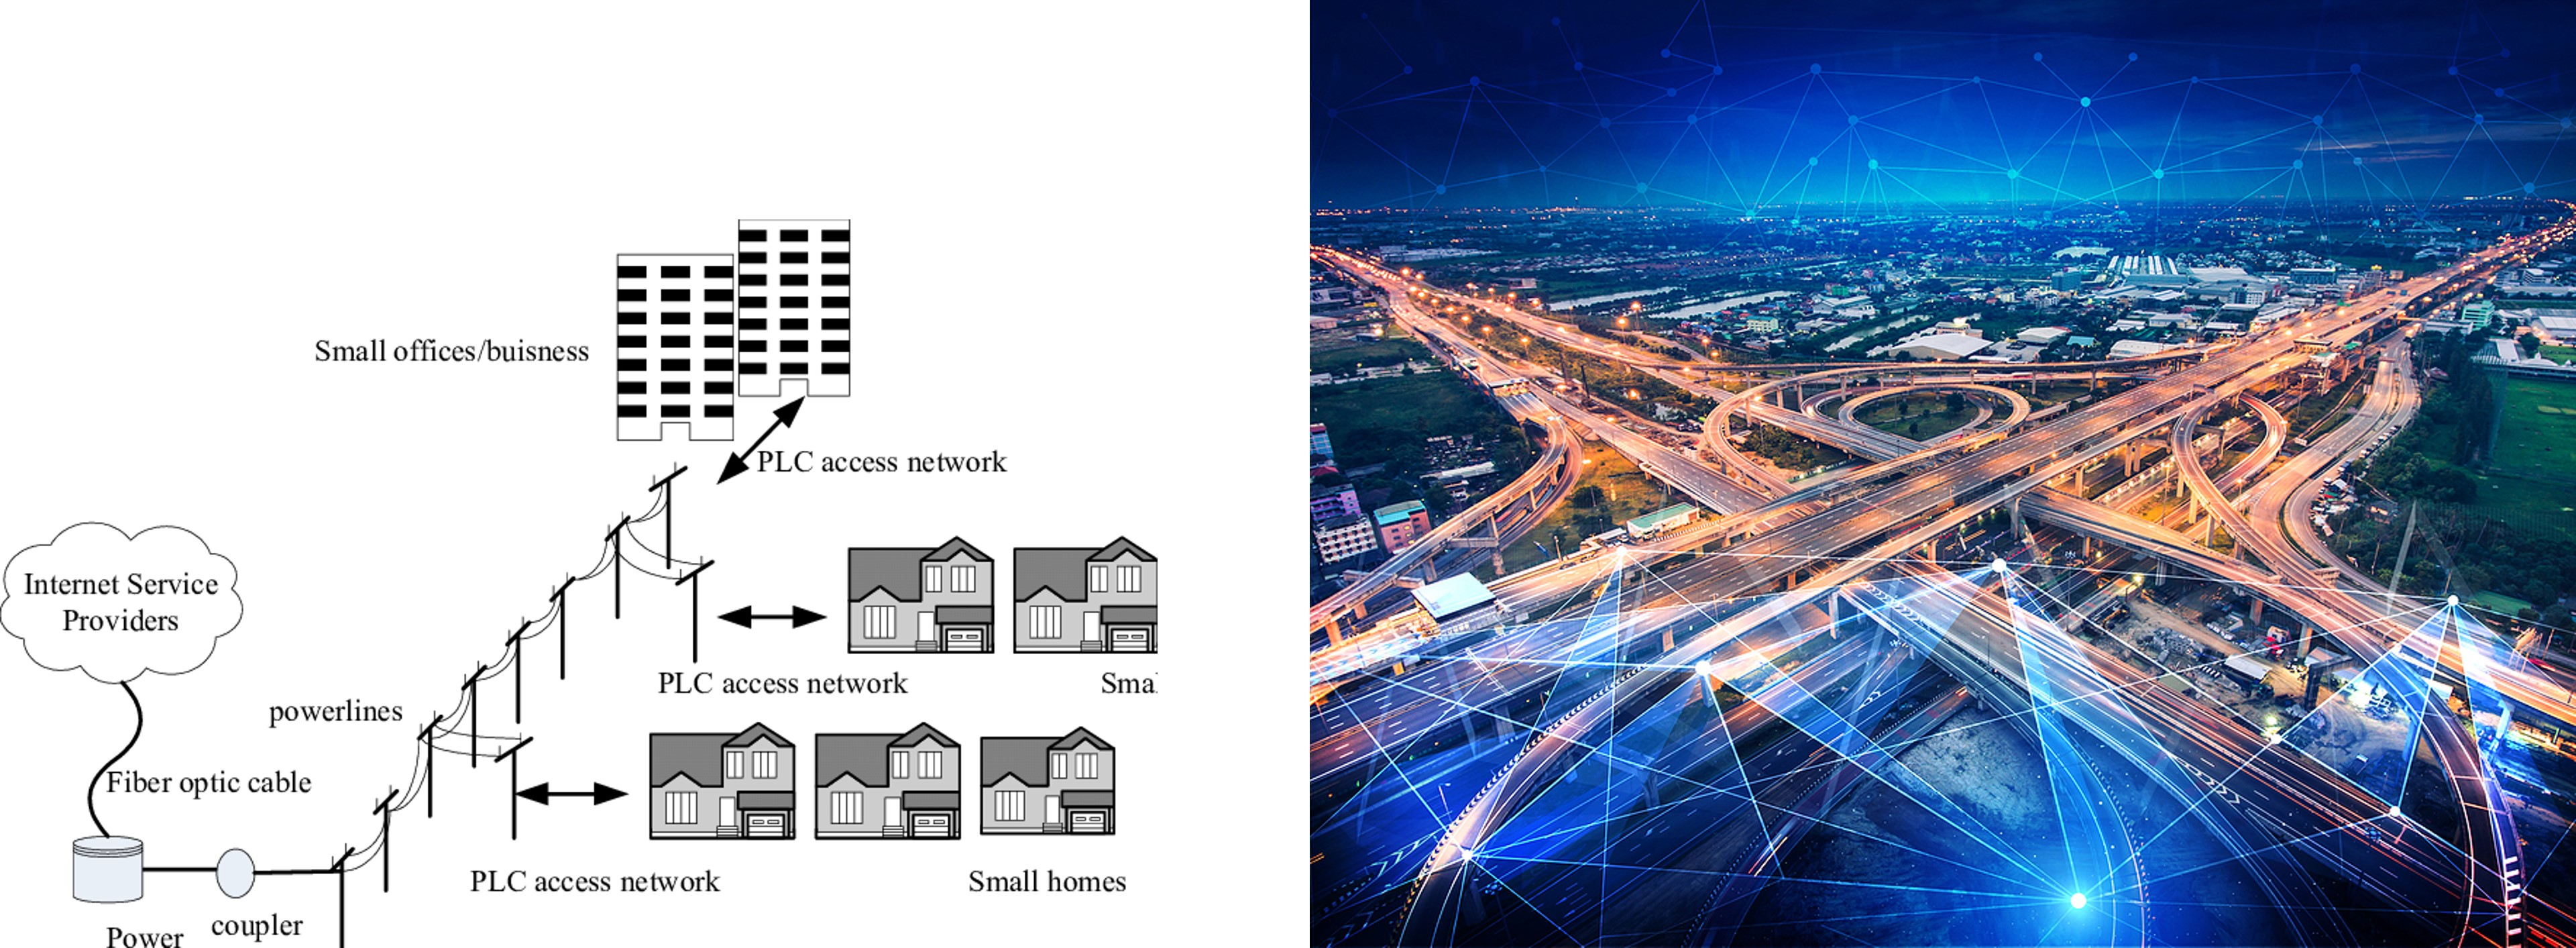
\includegraphics{./Images/supplychain/Relation with Transportation} 

}

\caption{Relation with Transportation}(\#fig:Figure 7.14)
\end{figure}

\hypertarget{SupplyChain-relation}{%
\section{How does it relate to Transportation?}\label{SupplyChain-relation}}

Whether ''First'' or ``Last Mile'', they both serve as connectors that either initiate or end a trip.
In Transportation, there are two types or trips being done:
The Movement of Goods
The Movement of People
The First Mile isn't as much of an issue when delivering goods compared to people\ldots{} more on this later.

\begin{figure}

{\centering 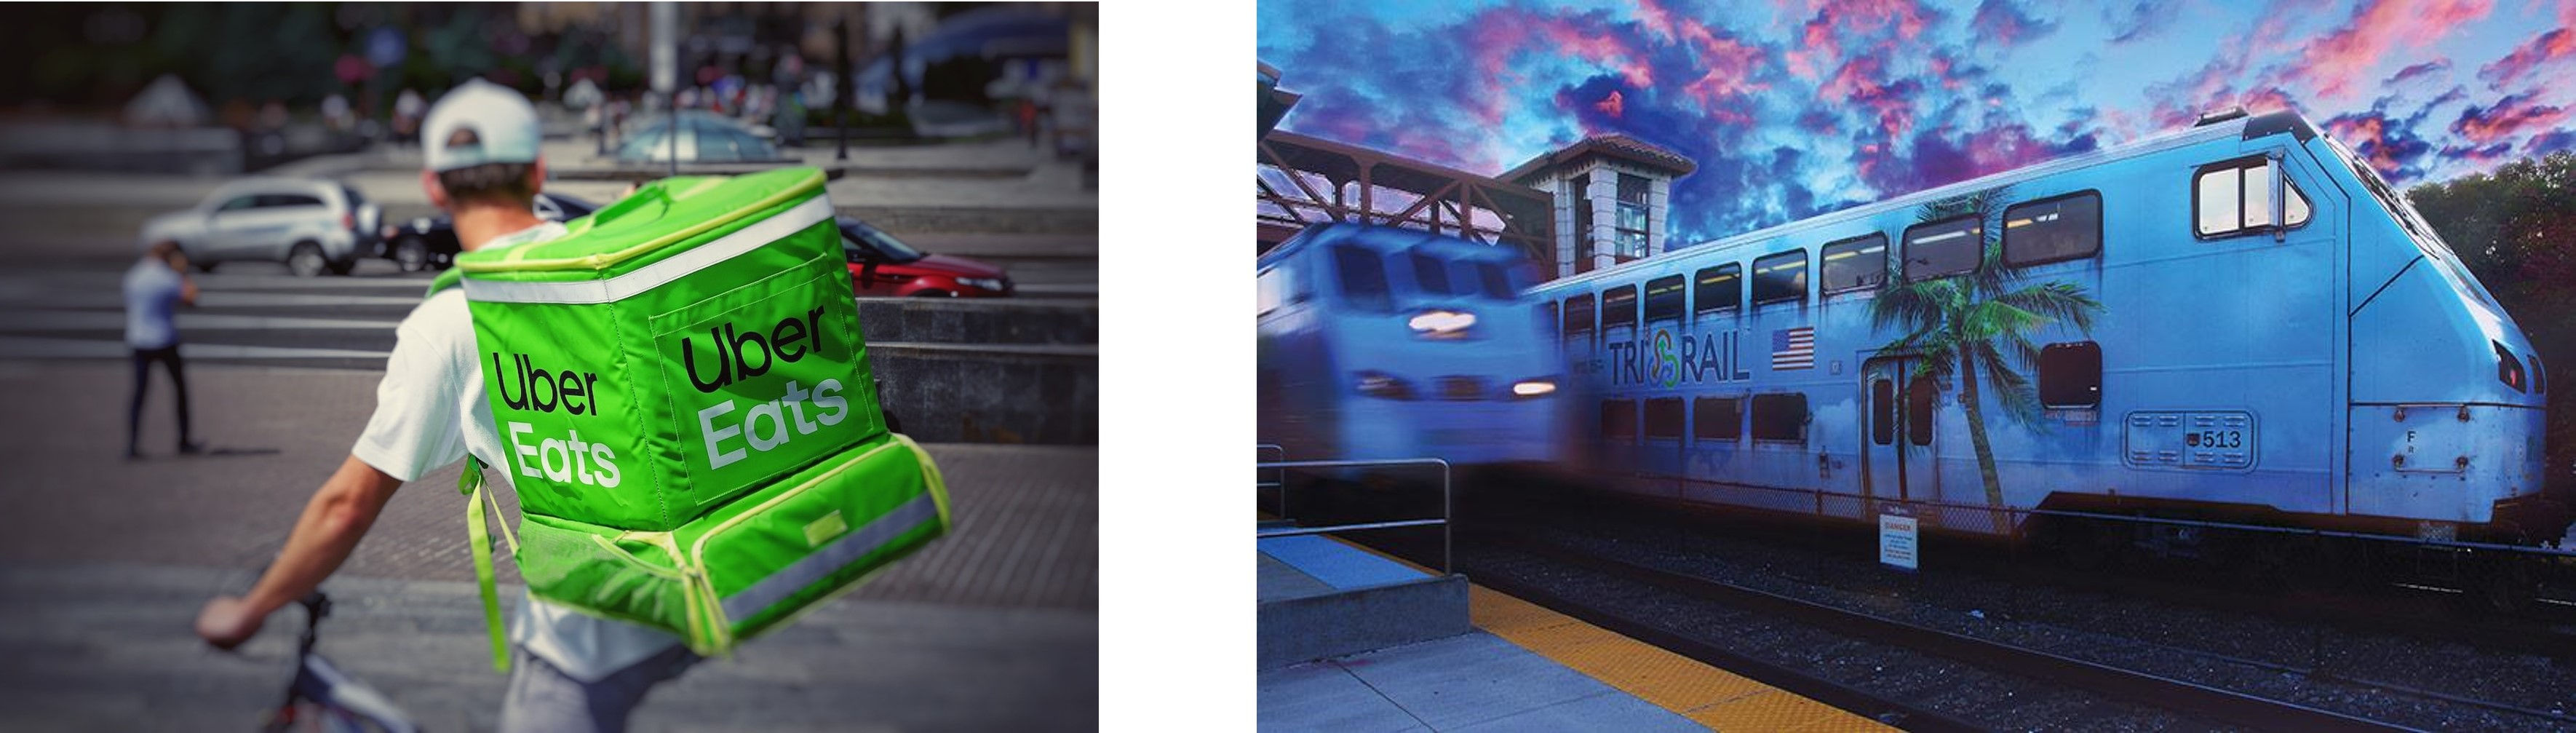
\includegraphics{./Images/supplychain/How does it relate to Transportation} 

}

\caption{How does it relate to Transportation}(\#fig:Figure 7.15)
\end{figure}

Movement of Goods

1.Last Mile regarding the movement of goods is the final step in the supply chain that moves goods from the distributor/facility to the costumer.
2.Last Mile usually involves parcel or small package carriers to deliver products
3.According to research done by straits, Last Mile Delivery market size is expected to reach \$123 Billion USD by 2030 from the \$40.5 Billion USD valuation given in 2021.
4.This is due to an increase in e-commerce and then COVID-19 further fueled the trend of ordering online.
5.The introduction of Omnichannel Supply Chains has also contributed to the market increase in Last Mile delivery.

6.In Supply Chain, traditionally the network is a Multichannel Supply Chain. This network would have departments grouped into stand alone silos with no interaction with one another.
Example: A retail company would have a brick-and-mortar store and an online store. Each store would have its own supply channel such as warehouse management and transportation system. The infrastructure would only serve that one channel
Since there is not overlap in the networks, overhead costs increase with less efficiency to move product.
7.Omnichannel Supply Chains, changes by integrating all networks to minimize cost and increase efficacy.
Example: The retail company, whether it's serving the brick-and-mortar store or the online store, the supply chain is designed to serve both channel simultaneously.
If a customer can't find an item in the brick-and-mortar store, they can order it online for the costumer. OR If the customer orders an Item online, they can choose to pick up the item at the brick-and-mortar store.

\#\#Challenges? \{\#SupplyChain-challenge\}
Movement of Goods
One more note on Omnichannel Supply Chains,
1.With the implementation of algorithms and predictive analytics, companies hope to be more efficient in delivering goods\ldots{} But there are consequences.\\
2.In a lecture presentation given by Charles H.W. Edwards (Professor of the Practice, Department of City and Regional Planning UNC -- Chapel Hill) to Florida Atlantic University's Fright Mobility Research Institute, Dr.~Edwards presented on companies urge to anticipate orders for the purpose of faster shipping.
3.E-commerce and online stores would look at trends generated by the number of clicks on their websites and then order products on the assumption that the consumer will eventually click the buy button.
4.The companies would order product before generating a sale and cause further unneeded stress for the First and Middle Mile, often\ldots{} the consumer would never click the buy button, but the product would already be shipped from the manufacture to the distribution hub.

5.Traffic Congestion and Parking are the main issues that affect Last Mile Deliveries.
6.Distribution hubs are usually located far from the cities in more rural areas.
Land is cheaper and available, more ample space for large trucks to move in and out of facilities.

7.But to move goods from the distribution hub to the final-destination (Last Mile), the challenge is traffic encountered in densely packed cities, accidents and other unforeseen events make delivery route optimization very difficult.\\
8.Finding parking in order to deliver goods can sometimes be difficult.

\hypertarget{SupplyChain-Soln}{%
\section{Solutions?}\label{SupplyChain-Soln}}

Movement of Goods
1.One way the industry can combat last mile challenges. Is by opening a secondary distribution hub outside the major city limits. Goods would go from the regional distribution center to this secondary distribution hub. Then the goods are closer to final-destination in the city.
2.Making the distance for the last mile smaller.
3.But the real solution comes from the type of vehicle used to distribute the the goods in the city
4.Proposed Solutions:
Delivery lockers, example: Amazon's storefront pickup locations.
Drone and robots.
Route optimization software

FMRI Research:
1.Sustainable Urban Freight Mobility Through Optimization of Logistics Facility Locations. FMRI Research Project.

This project considered to reevaluate freight providers traditional approach of positioning their distributions centers.
This is because the traditional approach causes traffic congestion, increased emissions and higher delay.
This project focused on a sustainable and cost-efficient approach by developing a a multi-objective framework for the facility location problem, NP-Hard optimization problem.
The model selects an optimal number of locations to create ``mini hubs'' inside the urban areas.
The trucks would arrive at the ``mini facilities and unload the goods.
The goods are then delivered (Last-Mile) via eco-friendly transportation modes (handcarts, bicycles, self-picked up) to the final destinations,
This project explores sustainable delivery solutions while simultaneously improving urban freight mobility.

\begin{enumerate}
\def\labelenumi{\arabic{enumi}.}
\setcounter{enumi}{1}
\tightlist
\item
  Integrate Autonomous delivery Vehicle Into Sustainable Urban Logistics Planning and Optimization.
  This project considered autonomous delivery vehicles as a novel approach to improve urban logistics and more specifically, improve the Last-Mile-Delivery.
  The reason this project was initiated is due to the current trend of sustainable urban distribution hubs which they are smaller logistic centers to be placed in the city.
  Studies show that drone delivery services are better suited for rural and suburban locations.
  But autonomous delivery vehicles (ADVs) are best suited for urban city centers.
  Specifically, ADVs should be used as ground bases delivery services to address the Last-Mile-Delivery.
  The reduce road traffic, no need for parking,
  The primary objective is to identify an urban logistic optimization model while minimizing operations cost and carbon footprint.
\end{enumerate}

\begin{figure}

{\centering 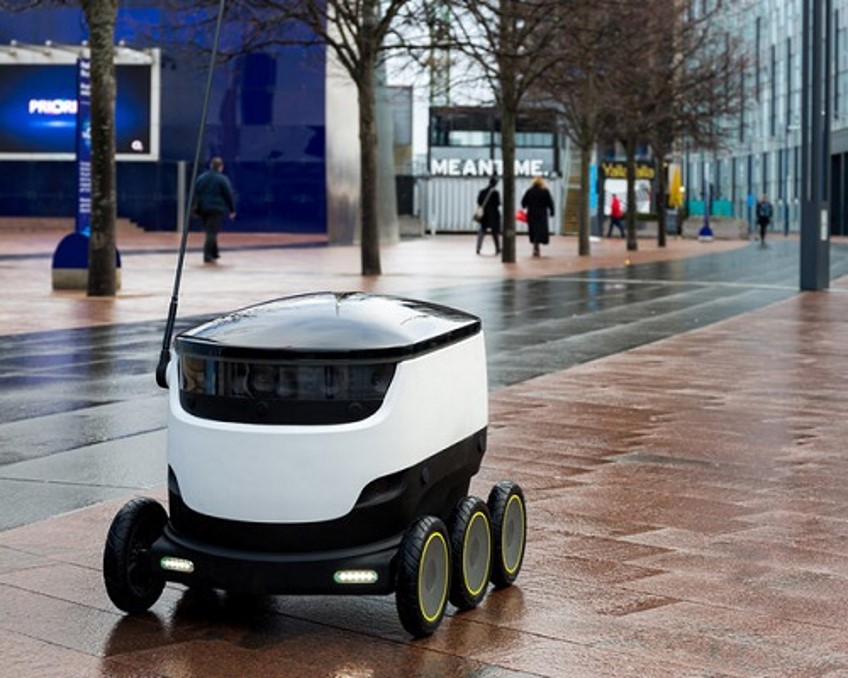
\includegraphics{./Images/supplychain/Autonomous Delivery Robot} 

}

\caption{Autonomous Delivery Robot}(\#fig:Figure 7.16)
\end{figure}

\hypertarget{SupplyChain-whatisrelation}{%
\section{How does it relate to Transportation?}\label{SupplyChain-whatisrelation}}

Movement of People
The First/Last Mile regarding the movement of people is the final step in the network to move people from the Main Mile to their destination.
Some of the modes that can be used for First/Last Mile:
Walking
Bikes
Local Transit
Taxis
Car Sharing
Micro transit
Zoning such as Complete Streets.

\begin{figure}

{\centering 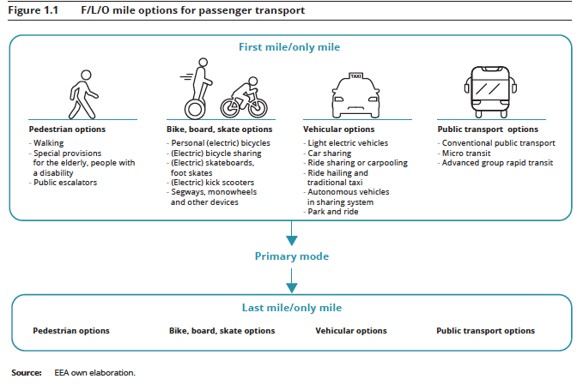
\includegraphics{./Images/supplychain/Passenger transport} 

}

\caption{Passenger transport}(\#fig:Figure 7.17)
\end{figure}

\hypertarget{SupplyChain-whatisFirstchallenges}{%
\section{Challenges}\label{SupplyChain-whatisFirstchallenges}}

Movement of People:
The challenges with the Last Mile regarding public transit is transit agencies failure to plan out major transit stops with major destinations.
Major destinations maybe a tourist attraction, employer, or residential neighborhoods.
The Census Bureau finds that 46\% of public transit commuters prefer to take buses over other forms of transportation\ldots{} however transit stops require commuters to walk the first or last leg of their trip.
The problem with walking is if the transit stop is more then ¼ mile away, nor the First/Last Mile, commuters may opt to not use public infrastructure.

\hypertarget{SupplyChain-solution}{%
\section{Solutions}\label{SupplyChain-solution}}

Movement of People:
Solutions include:
Updating or adding bike lanes
The City of Denton. Texas has produced a bike-sharing program that supports students from the University of Northern Texas campus and surrounding downtown area. The program is access via an app.\\
On-demand ride sharing
King County has created a on-demand ridesharing app that connects pedestrians to transit stops, The service area is mostly for Seattle.\\
On-demand micro transit
Complete Streets
Mobility Hubs (Broward County LRT concept)

\hypertarget{SupplyChain-haul}{%
\section{Long Haul, Short Haul}\label{SupplyChain-haul}}

\hypertarget{SupplyChain-whatishaul}{%
\section{What is Long Haul/Short Haul?}\label{SupplyChain-whatishaul}}

In Transportation, a trip can be classified as a long or short haul.
Often, various modes (land, air, sea) of transportation are utilized for long and short haul.
What determines a trip being a long or short haul is the type of good being transported and the location of the final destination.

\begin{figure}

{\centering 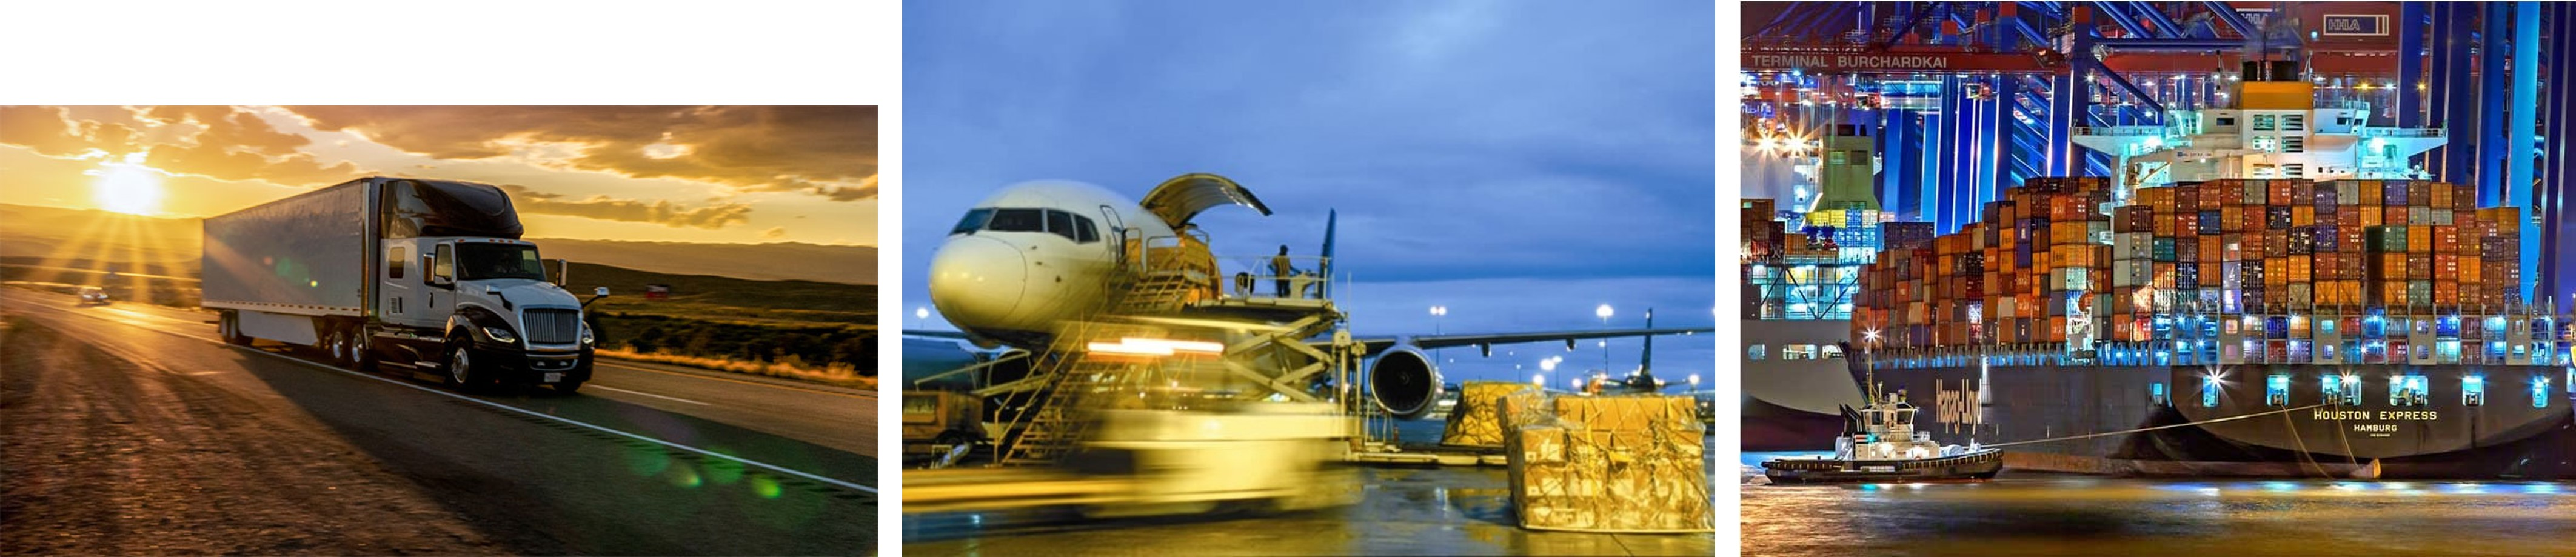
\includegraphics{./Images/supplychain/Long Haul and Short Haul} 

}

\caption{Long Haul and Short Haul}(\#fig:Figure 7.18)
\end{figure}

\#\#Land Transportation \{\#SupplyChain-landtpt\}

Long Haul:
Consists of larger trucks that can haul larger loads of goods across long distances.
Operate in a minimum radius of 250-miles, often between cities, states, or countries.
Typically found on interstates.

\begin{figure}

{\centering 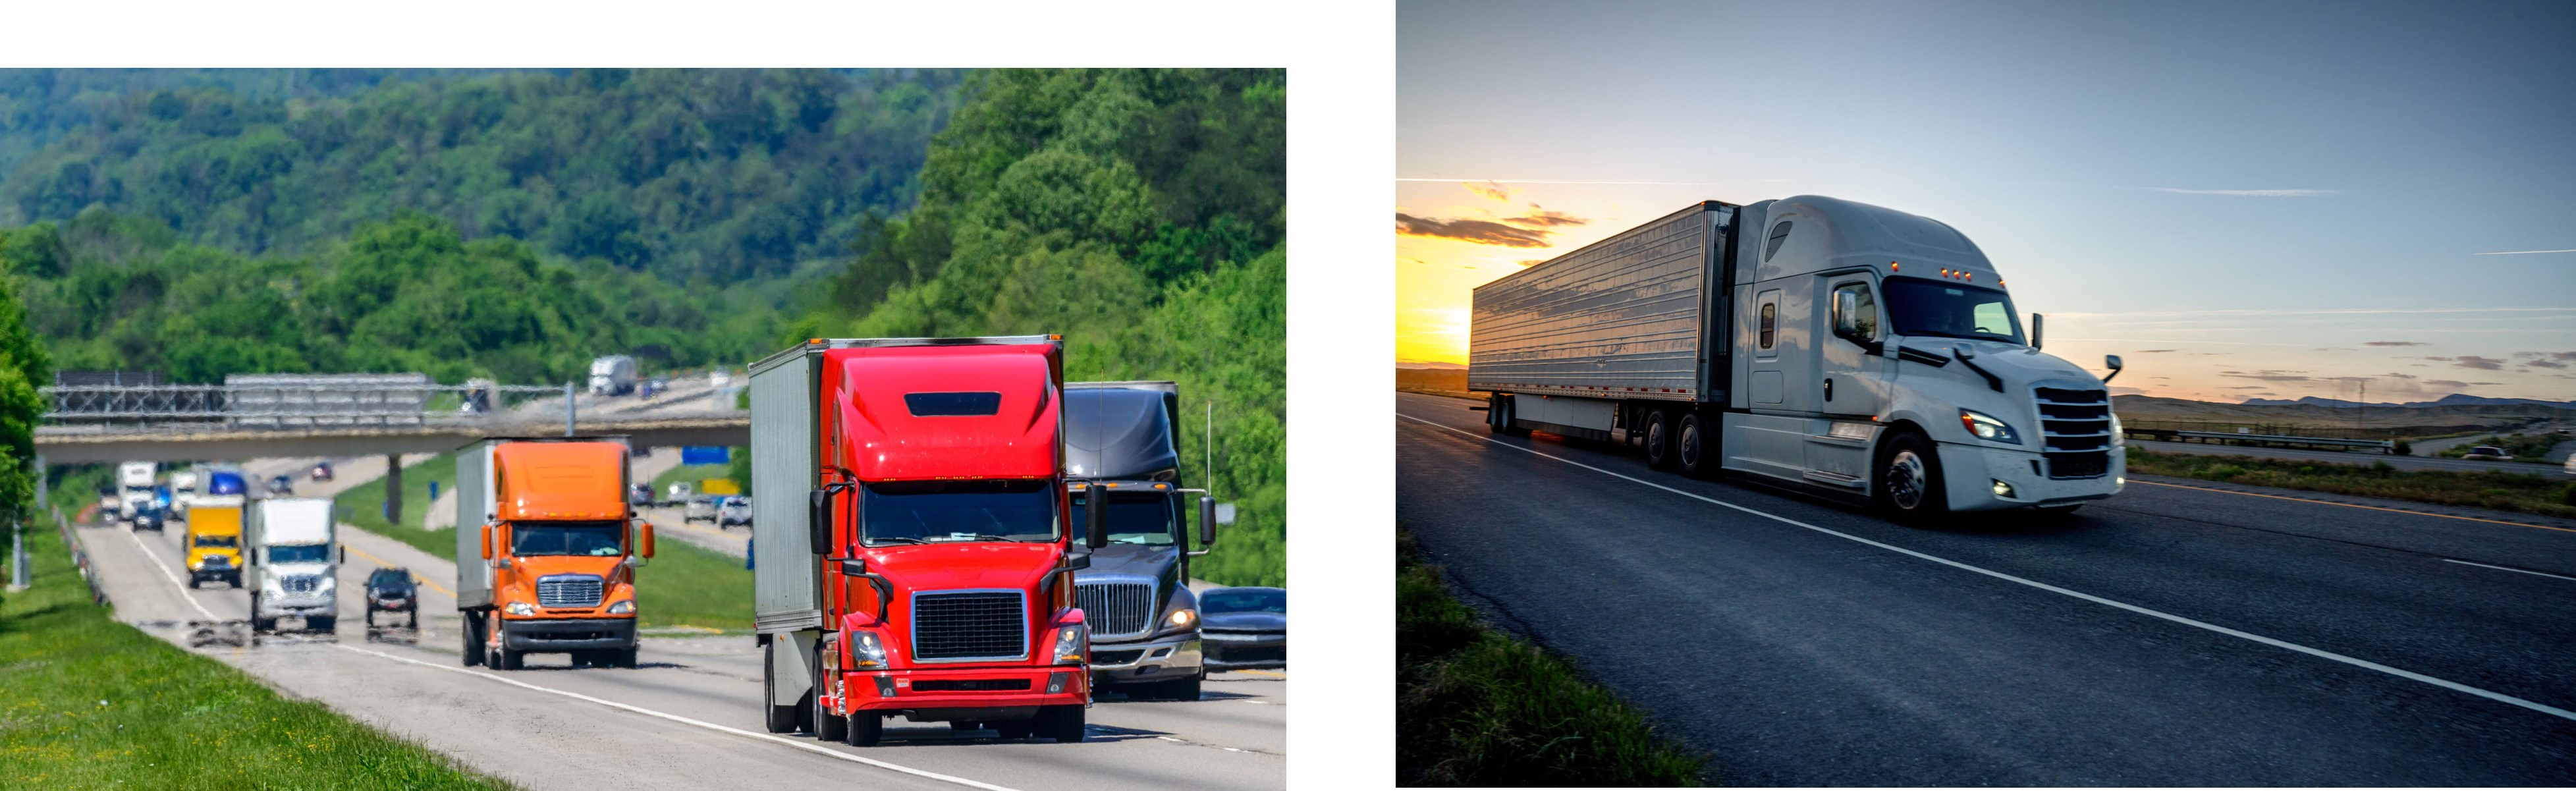
\includegraphics{./Images/supplychain/Long Haul} 

}

\caption{Long Haul}(\#fig:Figure 7.19)
\end{figure}

Short Haul:
Consists of small trucks that operate in a network within a 150-mile radius.
Usually operate within a city.
Examples: Delivery of materials to construction sites, Retail products from warehouses to brick-and-mortar stores.

\begin{figure}

{\centering 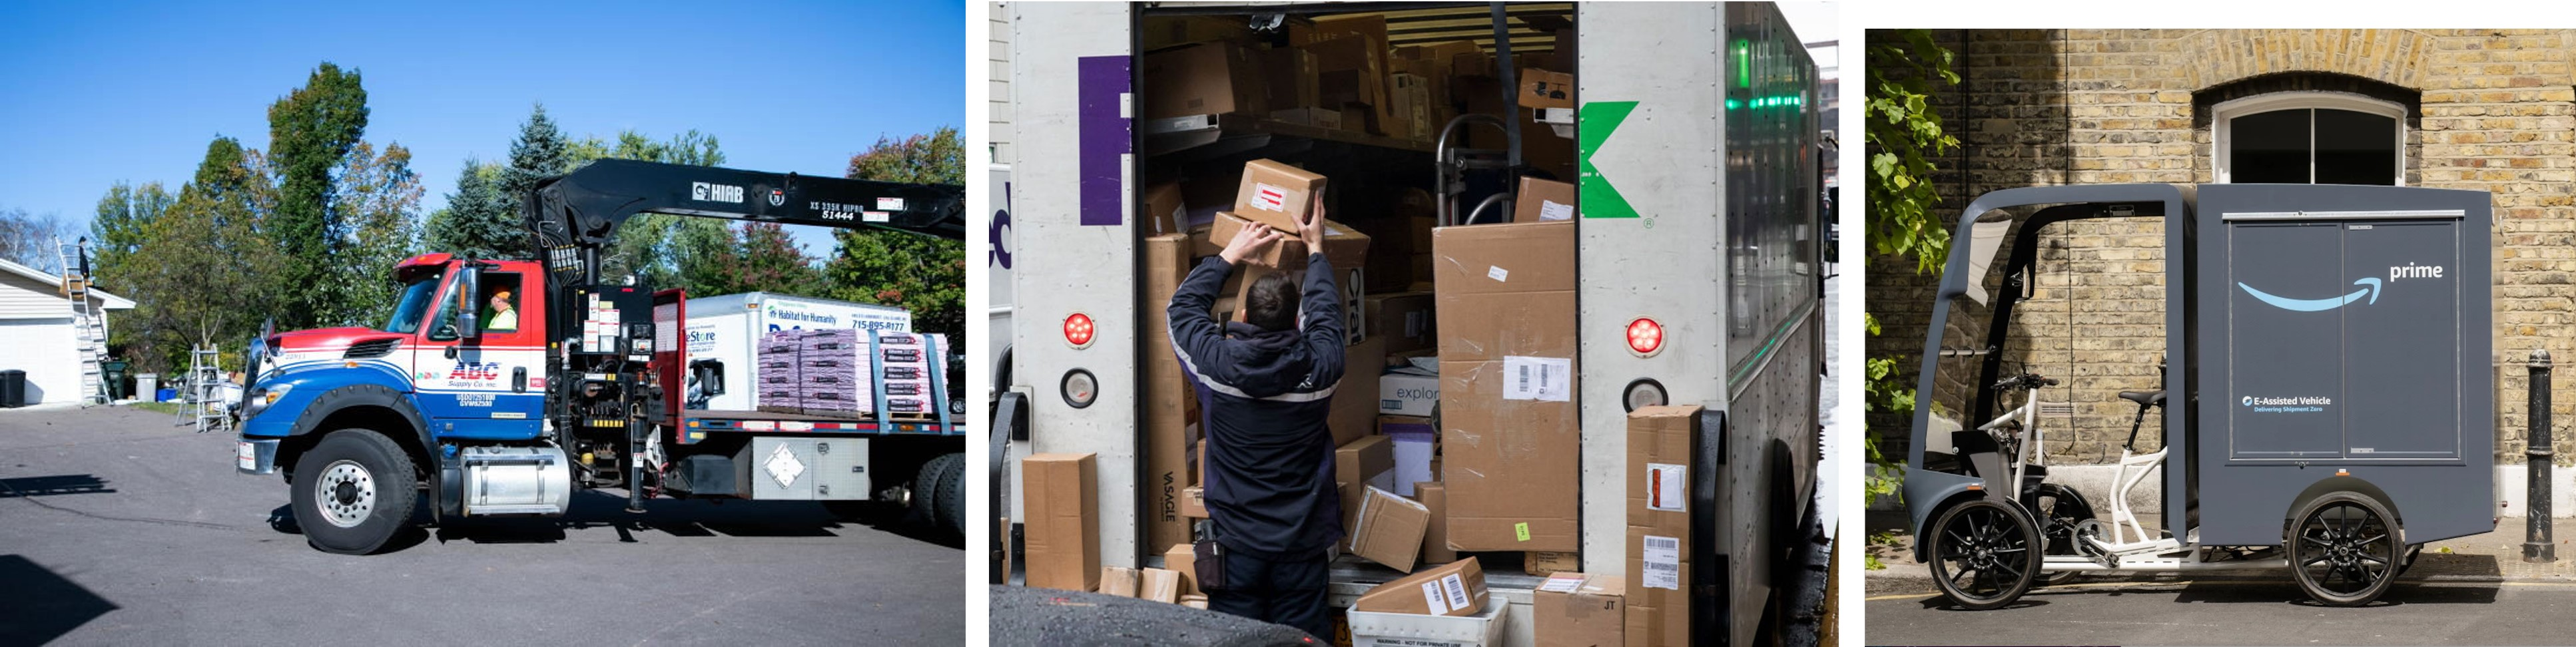
\includegraphics{./Images/supplychain/Short Haul} 

}

\caption{Short Haul}(\#fig:Figure 7.20)
\end{figure}

\hypertarget{SupplyChain-airtpt}{%
\section{Air Transportation}\label{SupplyChain-airtpt}}

Long Haul:
Commercial flights are categorized as short, medium, or long hauls, depending on the distances needed to travel.
Long haul flights consist of larger planes that can move goods or passengers across long distances.
Flight duration extends beyond but no less than 6 hours.
It can be for both connecting or non-stop flights
Pilots spend more days away then home.

\begin{figure}

{\centering 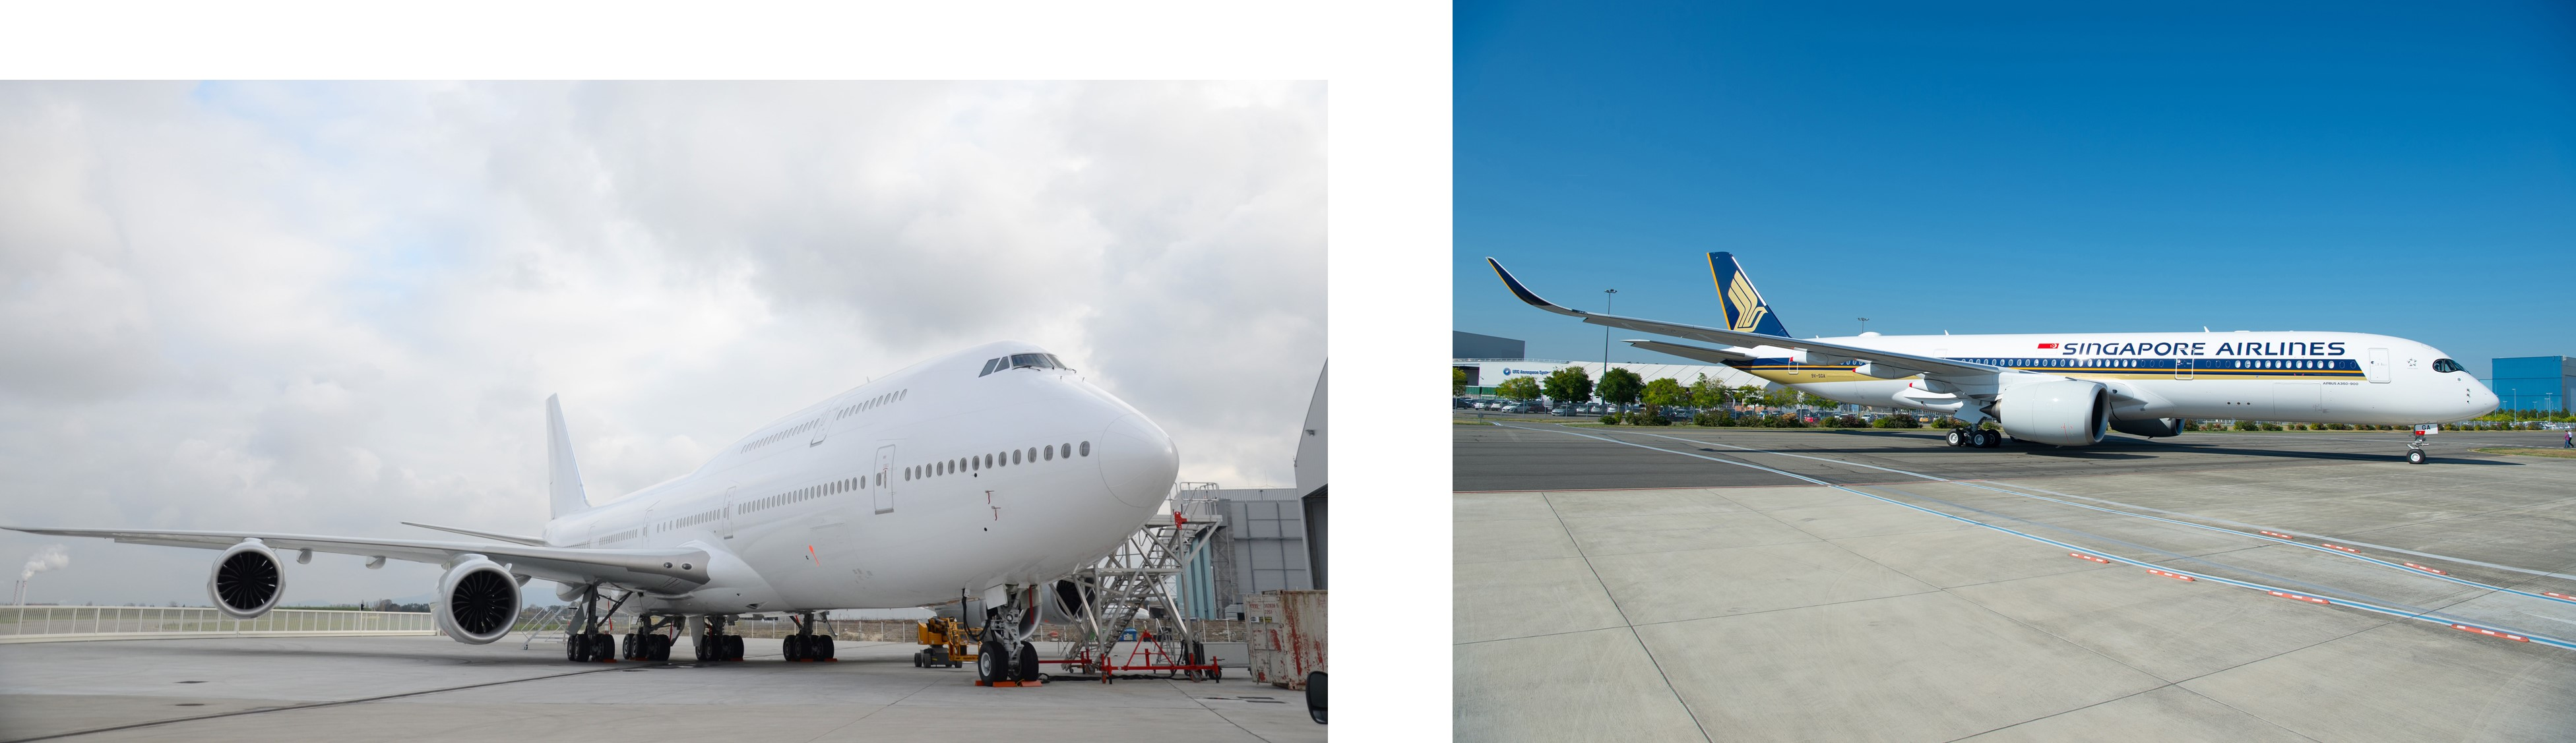
\includegraphics{./Images/supplychain/Air Transportation Long Haul} 

}

\caption{Air Transportation Long Haul}(\#fig:Figure 7.21)
\end{figure}

Ultra Long Haul:
Ultra long Haul (ULH) is an operational model that arose due to the Covid-19 virus.
ULH is proposed as a point-to-point service that, with a strong domestic ``feeder system'' would:
Require minimal adjustments to cope with Covid-19 or any future outbakes.
Produce higher seat-load factors and yields.
Produce more network flexibility.
Allow the ability to bypass densely populated hub airports.

\begin{figure}

{\centering 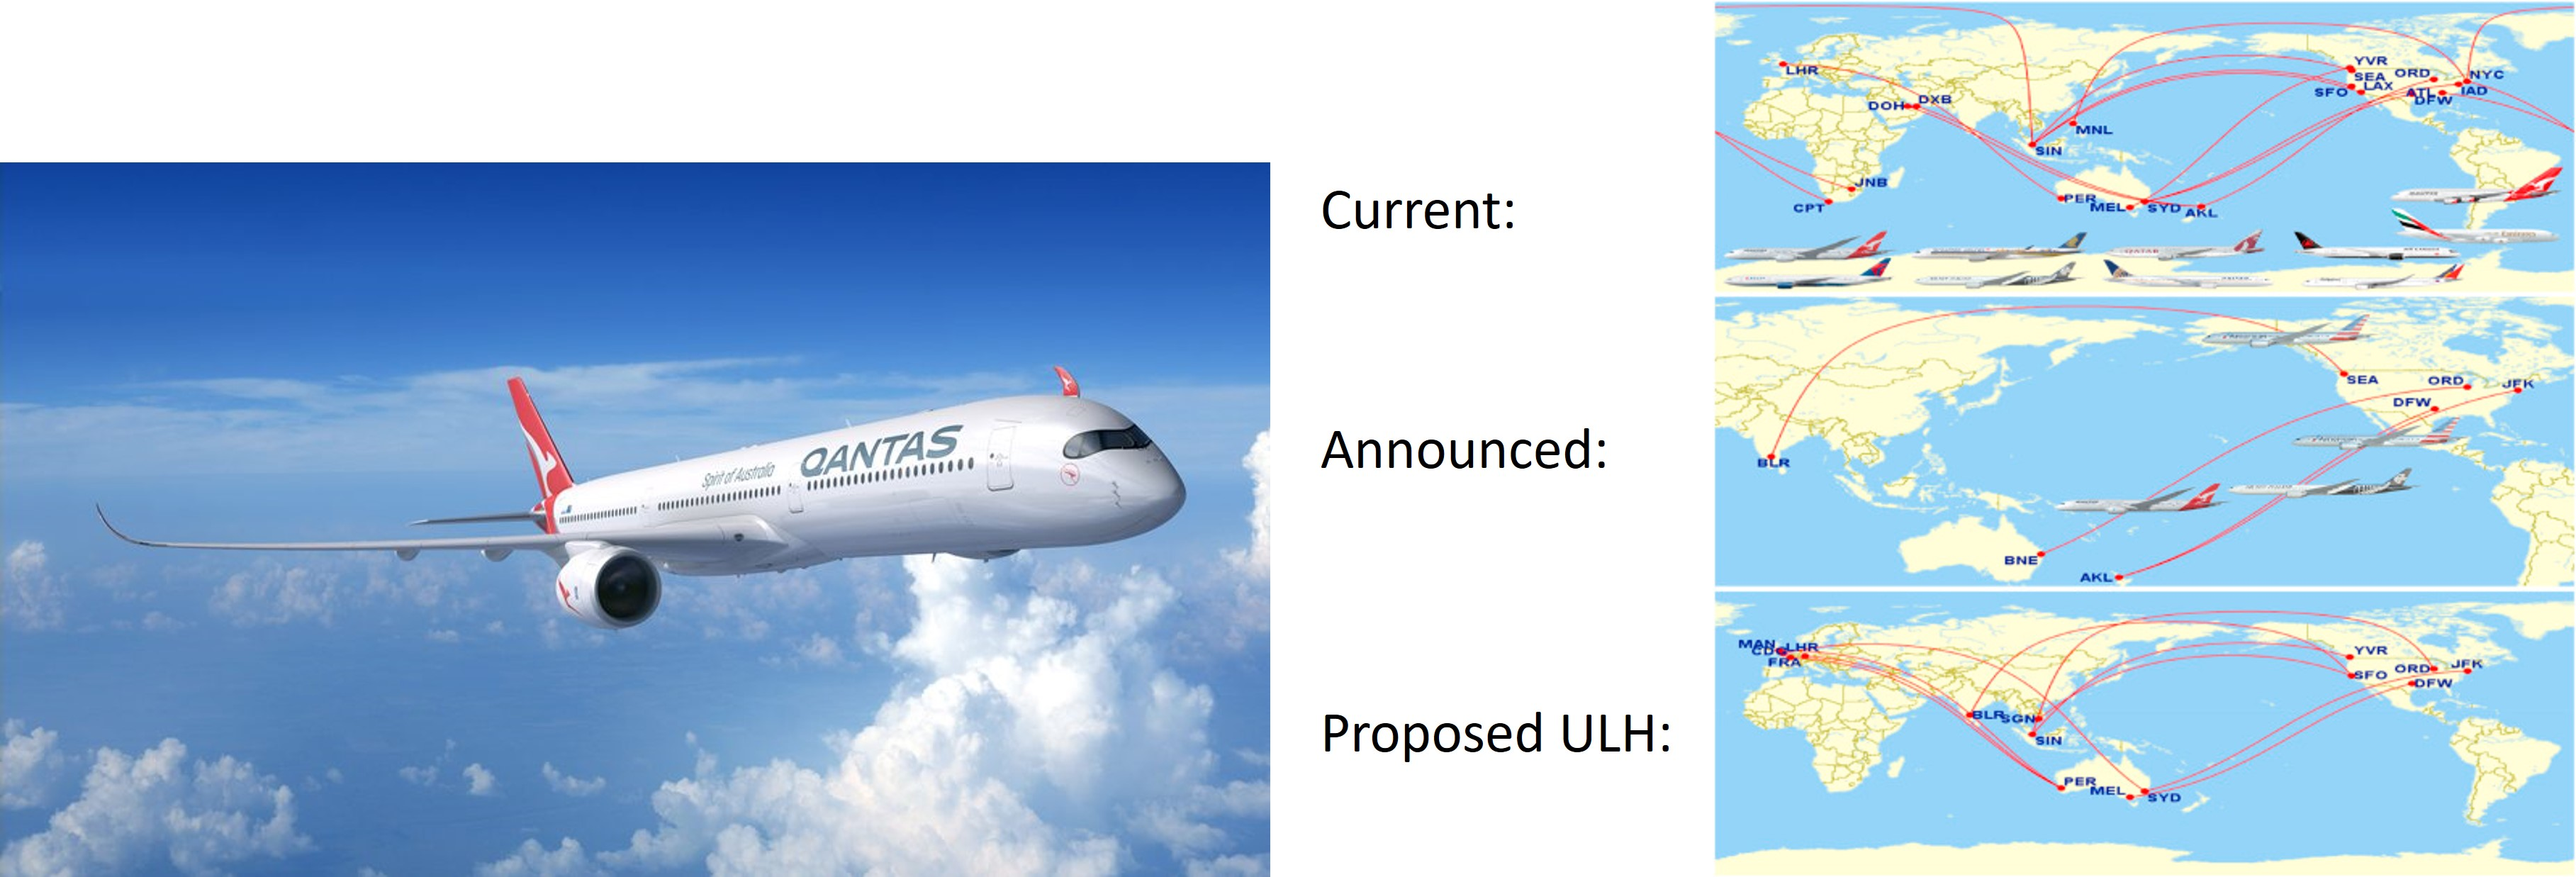
\includegraphics{./Images/supplychain/Ultra Long Haul} 

}

\caption{Ultra Long Haul}(\#fig:Figure 7.22)
\end{figure}

Short Haul:
Commercial flights categorized as short hauls, consist of smaller planes that are used in short but more frequent flights.
Flight duration lasts between 30 minutes to 3 hours.
Pilots make several trips a day and come back the same day.

\begin{figure}

{\centering \includegraphics{./Images/supplychain/Air Transportation Short Haul} 

}

\caption{Air Transportation Short Haul}(\#fig:Figure 7.23)
\end{figure}

\hypertarget{seaport}{%
\chapter{Seaport Operation}\label{seaport}}

\hypertarget{seaport-reefer}{%
\section{Reefer Units}\label{seaport-reefer}}

The term ``Reefer'' refers to a refrigerated container used to transport perishable goods.

While these units are used throughout most supply chains, they are especially important within marine settings as food often travels hundreds of miles before reaching consumers.

\begin{figure}

{\centering \includegraphics{./Images/seaport operation/Reefer Unit} 

}

\caption{Reefer Unit}(\#fig:Figure 8.1)
\end{figure}

\hypertarget{seaport-containers}{%
\section{Types of Reefer Containers}\label{seaport-containers}}

There are three typical types of Reefer Containers. Each have their own benefits and drawbacks.

\begin{figure}

{\centering \includegraphics{./Images/seaport operation/Types of Reefer Containers} 

}

\caption{Types of Reefer Containers}(\#fig:Figure 8.2)
\end{figure}

\hypertarget{seaport-work}{%
\section{How does a Reefer Container work?}\label{seaport-work}}

Reefer containers maintain the desired temperatures by channeling air under and around the cargo through T-shaped decking.

Reefer control units allow for the setting and adjustment of other parameters such as humidity, ventilation and atmosphere which varies between cargos.

Power supply is sustained through either portable generators or the vessel's power outlet.

\begin{figure}

{\centering \includegraphics{./Images/seaport operation/Reefer Container} 

}

\caption{Reefer Container }(\#fig:Figure 8.3)
\end{figure}

\hypertarget{seaport-necessary}{%
\section{Why are they necessary?}\label{seaport-necessary}}

The usage of reefer units has greatly influenced how we manage supply chains and what can be shipped.

Benefits of reefer units include:
Longer product shelf life
Diversification of shippable cargo
Durable enough to remain operational in harsh marine environments
Manufactured in multiple standard dimensions and can be partitioned to diversify cargo within individual containers
Cargo does not require immediate cold storage upon arrival to destination
\#\# Industry Regulations \{\#seaport-regulation\}

To prevent practices during transportation that create food safety risks, the FDA creates various rules and regulations. The Sanitary Transportation of Human and Animal Food Rule aims to address the failure to properly refrigerate food, inadequate cleaning of vehicles between loads, and failure to properly protect food.

Additionally, global organizations uphold and promote a higher standard for product quality and safety in conjunction with the rules set forth by the FDA.

\begin{figure}

{\centering \includegraphics{./Images/seaport operation/Industry Regulation} 

}

\caption{Industry Regulation}(\#fig:Figure 8.4)
\end{figure}

\hypertarget{seaport-20ft40ft}{%
\section{20ft and 40ft Containers}\label{seaport-20ft40ft}}

\hypertarget{seaport-freight}{%
\section{The Modern Freight Container}\label{seaport-freight}}

The term ``freight transportation'' conjures images of boats or trains filled to the brim with modern day shipping containers, but the movement of merchandise has not always been this simple.

Prior to the 18th century, freight was handled manually as break bulk cargo. In other words each item was individually accounted for and transferred between carriers- a rather inefficient method.

Malcolm McLean patented the first standardized shipping container in 1956. These steel containers were designed to be robust and reliable.

\hypertarget{seaport-modern}{%
\section{Impact of Modern Containers on Seaport Operations}\label{seaport-modern}}

Containerization, the process unitization of cargoes in exports, greatly impacted shipping operations.

The advent of the modern container brought a decline of inland ports as they were no longer able to support massive container ships. Seaports built along deep waterways became the predominant terminal for shipping.

With the use of containers, products were safely sealed reducing pilfering and overall damages.

Containers also reduced the labor requirements within ports as cranes took the place of large longshoremen crews.

Overall, there was a rise in efficiency and speed of export accompanied by a decrease in shipping costs.

\begin{figure}

{\centering \includegraphics{./Images/seaport operation/Containers} 

}

\caption{Containers}(\#fig:Figure 8.5)
\end{figure}

\hypertarget{seaport-size}{%
\section{ISO Standard: Container Sizes}\label{seaport-size}}

The International Organization for Standardization (ISO) sets the standard for shipping container sizes in addition to other practices. These standards can all be found on the ISO website.

Typically, containers are either 20' or 40' for general purposes but occasionally other sizes may be used such as the one outlined in red above. ISO 668:2020 outlines the classification, dimensions and ratings for series 1 freight containers.

\begin{figure}

{\centering \includegraphics{./Images/seaport operation/Container Size} 

}

\caption{Container Size}(\#fig:Figure 8.6)
\end{figure}

\hypertarget{seaport-markings}{%
\section{ISO Standard: Container Markings}\label{seaport-markings}}

All markings on the exterior of a shipping container are done in accordance with ISO Standard 6346:2022.

The bulk of the information can be found on the door side of the shipping container.

\begin{figure}

{\centering \includegraphics{./Images/seaport operation/Container Markings} 

}

\caption{Container Markings}(\#fig:Figure 8.7)
\end{figure}

The container numbers consists of owner codes, equipment categories, serial numbers and check digits. The container numbers must be displayed on all sides of the container.

The size and type code is usually below the container numbers. The first character of the code indicates the length of the container, the second represents the width/height, and the third and fourth character indicates the container type.

Prior to shipment, containers must have a safety approval per the international convention for safe containers (CSC). This approval is indicated by the CSC Plate located on the outer left door of the container. Typically the CSC Plate is now combined with the customs plate and any other plates required for international trade- collectively known as the Combined Data Plate.

\begin{figure}

{\centering \includegraphics{./Images/seaport operation/ISO Standard Container Markings} 

}

\caption{ISO Standard Container Markings}(\#fig:Figure 8.8)
\end{figure}

\hypertarget{seaport-types}{%
\section{Types of Containers}\label{seaport-types}}

\begin{enumerate}
\def\labelenumi{\arabic{enumi}.}
\tightlist
\item
  Dry Storage Containers:
\end{enumerate}

These containers are some of the most common in the industry. They are designed to transport dry goods. These containers do not allow for temperature controls, so they are not suited for moving food or chemicals that require refrigeration.

\begin{enumerate}
\def\labelenumi{\arabic{enumi}.}
\setcounter{enumi}{1}
\tightlist
\item
  Flat Rack Containers:
\end{enumerate}

Flat rack containers are ideal for shipping boats, cars and other heavy machinery. These containers do not have a top and two of their sides may be optional. Often times, the sides of the containers are either collapsible or detachable.

\begin{figure}

{\centering \includegraphics{./Images/seaport operation/Types of Containers} 

}

\caption{Types of Containers}(\#fig:Figure 8.9)
\end{figure}

\begin{enumerate}
\def\labelenumi{\arabic{enumi}.}
\setcounter{enumi}{2}
\tightlist
\item
  Open Top Containers:
\end{enumerate}

These containers have an open top to allow for ease of bulk cargo loading. During shipping a roof structure may be secured to the container via ropes to protect against precipitation.

\begin{enumerate}
\def\labelenumi{\arabic{enumi}.}
\setcounter{enumi}{3}
\tightlist
\item
  Open Side Containers:
\end{enumerate}

Open side containers are used for cargo that would otherwise not fit through the standard door openings of a dry storage container. The side swings open as if it was made of two large doors, but it can still be secured to protect the merchandise inside.

\begin{enumerate}
\def\labelenumi{\arabic{enumi}.}
\setcounter{enumi}{4}
\tightlist
\item
  Tanks:
\end{enumerate}

Tanks are designed to retain liquids, especially fuels. They are typically constructed out of anti-corrosive materials because of the harsh chemicals they carry.

\begin{enumerate}
\def\labelenumi{\arabic{enumi}.}
\setcounter{enumi}{5}
\tightlist
\item
  Refrigerated Containers:
\end{enumerate}

Refrigerated containers have temperature controls so goods can be kept at a specific temperature during transport. They are well insulated to ensure that the climate remains consistent. These containers allowed for a wider range of shippable cargo.

\hypertarget{seaport-packed}{%
\section{How are containers packed?}\label{seaport-packed}}

\begin{figure}

{\centering \includegraphics{./Images/seaport operation/Container Packing} 

}

\caption{Container Packing}(\#fig:Figure 8.10)
\end{figure}

\hypertarget{seaport-lading}{%
\section{Bill of lading}\label{seaport-lading}}

The Bill of Lading and the Freight Bill are two of the most important forms when shipping containers.

The Bill of Lading is essentially a shipping contract which describes the origin and destination of the merchandise, the quantity, the description of goods and the cost of shipment. This document is legal proof of the shipment and can be used during legal proceedings.

The Freight Bill is the invoice for the shipping from origin to destination. This document includes all the details of shipment and is signed by both the shipper and carrier. Unlike the bill of lading, this document cannot be used during legal disputes as proof of shipment.

\begin{figure}

{\centering \includegraphics{./Images/seaport operation/Bill of Lading} 

}

\caption{Bill of Lading}(\#fig:Figure 8.11)
\end{figure}

\hypertarget{planning}{%
\chapter{Planning, Design, Operations Management Organizations}\label{planning}}

\hypertarget{planning-DOT}{%
\section{State DOTs}\label{planning-DOT}}

Introduction
1.Each state has its own department of transportation, that is responsible for transportation planning, design, management and operations that act in accordance with regulations and guidelines.
2.These regulations and guidelines establish consistency across the nation, allowing for each state to navigate through their own environmental, geographical, and geological challenges

\begin{figure}

{\centering \includegraphics{./Images/planning design/State DOTs} 

}

\caption{State DOTs}(\#fig:Figure 9.1)
\end{figure}

\hypertarget{planning-plan}{%
\section{Planning}\label{planning-plan}}

1.Each state has its own transportation planning office, and it is usually divided into subcategories
2.For example, the Florida Department of Transportation, has a central planning office, that has four subcategories: policy planning, forecasting and trends, system implementation, and performance.

\begin{figure}

{\centering \includegraphics{./Images/planning design/planning} 

}

\caption{planning}(\#fig:Figure 9.2)
\end{figure}

\hypertarget{planning-process}{%
\section{FDOT Planning Processes}\label{planning-process}}

Florida Transportation Plan (FTP)
Strategic Intermodal System (SIS)
Planning Studies
Access Management
Interchange Access Request (IAR)
Highway Capacity/Level of Service (LOS)
Project Traffic Forecasting
Site Impact Analysis
Shared Use Non-motorized (SUN) Trail network
Statistics, Measures, and Trends
Performance Measures

Strategic Intermodal System (SIS):

This network establishes a competitive market for the states economy,and improves the functionality of the transportation system considering heavy congested areas that surround highways, trails, waterways, ports, and airports.

Florida Transportation Plan (FTP):

This plan has three subcategories: the FTP vision element, the FTP policy element, and the FTP implementation element. Each aspect of this plan is purposed to outline the future of the Florida transportation system, develop technology based consumer application, and further implement performance measures for state, regional, and local agencies.

\begin{figure}

{\centering \includegraphics{./Images/planning design/planning process} 

}

\caption{planning process}(\#fig:Figure 9.3)
\end{figure}

\hypertarget{planning-design}{%
\section{Design}\label{planning-design}}

Each state has its own transportation design team located in the state department of transportation.
The office of design's purpose is to innovatively supply transportation solutions to problems faced by the community.
The Florida Department of Transportation has a design team that consistent of three subcategories: Production Support, Roadway Design, and Structures Design.
This team establishes policies, regulations, and standards for structures, highways, and bridges.

\hypertarget{planning-operation}{%
\section{Operation Management}\label{planning-operation}}

FDOT Operations:

ITS Communications
Managed Lanes
Management and Deployment
Software and Architecture
Statewide Arterial Management Program (STAMP)
Traffic, Incident Management (TIM)/Commercial Vehicle Operations (CVO)
Traffic Systems

\begin{figure}

{\centering \includegraphics{./Images/planning design/operation management} 

}

\caption{operation management}(\#fig:Figure 9.4)
\end{figure}

Traffic, Incident Management (TIM):

This program establishes new methods to quickly and efficiently identify and respond to crashes. This program trains first responders, and Rapid Incident Scene Clearance (RISC) on clearing the incident or crash to prevent further hazardous consequences.

Managed Lanes:

This program establishes express lanes, and additional supplemental lane mobility that allows for the driver to have an efficient driving experience, while also supplying accurate data that can further shape the future of the transportation system

\hypertarget{planning-freight}{%
\section{Freight Plan}\label{planning-freight}}

As the nation has grown, so has the freight transportation industry. Freight transportation is essential to development, supporting population expansion and economic activity, enabling dramatic growth, and incorporating multiple components that employ millions.

1.A freight plan is a blueprint for action that identifies the implementation steps that will solve freight needs and issues.

2.In order to create an actionable plan, a client must first determine how the plan will be implemented when it's finished. Then, working backwards, the plan will include the pieces needed to become a reality.

3.The U.S. federal government requires state departments of transportation and metropolitan planning organizations to develop freight plans, and if done right, those plans can have great benefit for a community or state.

4.A well thought out freight plan supports economic development, addresses private sector demands, matches funding and financing options for projects, and provides justification and transparency for investment decisions.

\hypertarget{planning-freightplanning}{%
\section{How Can A Client Get The Most Out Of Freight Planning?}\label{planning-freightplanning}}

Freight plans are customized to fit the needs of each client.
Freight plans generally focus on these topics:

Mobility (efficient and reliable movement)
Economic development
Infrastructure: maintaining existing assets and developing new capacity
Safety
Environmental protection
Equity and community

\hypertarget{planning-guidance}{%
\section{Purpose of the Guidance on State Freight Plans}\label{planning-guidance}}

Provide States with information on the required elements.
Provide a template that reflects those statutory requirements.
Recommend approaches and information (optional elements) States may include.
Provide suggestions and encourage States to establish
State Freight Advisory Committees to benefit State freight planning.

\hypertarget{planning-strategicplan}{%
\section{National Freight Strategic Plan}\label{planning-strategicplan}}

\begin{enumerate}
\def\labelenumi{\arabic{enumi}.}
\tightlist
\item
  Safe, reliable, and efficient freight transportation boosts exports, enhances commerce, and powerseconomic growth. Our robust national multimodal freight system supports our economy by lowering costs to businesses and consumers and boosting the competitiveness of American goods abroad. The safe and efficient movement of goods through our freight system is a top priority for the U.S Department of Transportation (U.S. DOT).
\end{enumerate}

2.This National Freight Strategic Plan defines the U.S. DOT's vision and goals for the national multimodal freight system, assesses the conditions and performance of the freight system and barriers to freight system performance, and defines strategies to achieve its vision and goals. The Plan was developed through a multiagency effort involving extensive consultation with freight stakeholders in both the public and private sectors.

3.The Department will use this Plan to guide national freight policy, programs, initiatives, and investments; inform State freight plans; identify freight data and research needs; and provide a framework for increased cross-sector, multijurisdictional, and multimodal coordination and partnerships.

\hypertarget{planning-vision}{%
\section{Vision}\label{planning-vision}}

The freight transportation system of the United States will strengthen our economic competitiveness with safe and reliable supply chains that efficiently and seamlessly connect producers, shippers, and consumers in domestic and foreign markets.

\begin{figure}

{\centering \includegraphics{./Images/planning design/vision} 

}

\caption{vision}(\#fig:Figure 9.5)
\end{figure}

\hypertarget{planning-policy}{%
\section{National Freight Policy Strategic Goals}\label{planning-policy}}

\begin{figure}

{\centering \includegraphics{./Images/planning design/Strategic Goals} 

}

\caption{Strategic Goals}(\#fig:Figure 9.6)
\end{figure}

\#Enforcement and Safety Organizations\{\#safety\}

\hypertarget{safety-federal}{%
\section{Federal Motor Carrier Safety Administration}\label{safety-federal}}

Introduction

What is the Federal Motor Carrier Safety Administration?

1.The Federal Motor Carrier Safety Administration (FMCSA) is a governmental agency that is responsible for supervising and regulating motor carriers.
2.The FMCSA has established its headquarters in Washington D.C, while it oversees commercial driver licensing, bus companies and commercial trucking.

\begin{figure}

{\centering \includegraphics{./Images/Enforcement and Safety Organizations/Federal Motor Carrier Safety Administration} 

}

\caption{Federal Motor Carrier Safety Administration}(\#fig:Figure 10.1)
\end{figure}

\hypertarget{safety-evolution}{%
\section{Evolution}\label{safety-evolution}}

The FMCSA was established through the Motor Carrier Safety Improvement Act of 1999 on January 1, 2000 by the United States Department of Transportation
The FMCSA now has over 1,000 employees stationed across the country
One of the most recent additions of regulations includes the FMCSA Clearinghouse, which provides the ability to prohibit drivers to operate vehicles based on alcohol and drug testing and violations.

\begin{figure}

{\centering \includegraphics{./Images/Enforcement and Safety Organizations/DOT} 

}

\caption{DOT}(\#fig:Figure 10.2)
\end{figure}

\hypertarget{safety-Purpose}{%
\section{Purpose}\label{safety-Purpose}}

What is the purpose of the Federal Motor Carrier Safety Administration?

The purpose of this administration is enforce, regulate, and adjust the standard operating procedures for motor carrier vehicles to prevent and reduce crashes.

\begin{figure}

{\centering \includegraphics{./Images/Enforcement and Safety Organizations/Purpose} 

}

\caption{Purpose}(\#fig:Figure 10.3)
\end{figure}

\hypertarget{safety-Programs}{%
\section{Programs}\label{safety-Programs}}

What does the Federal Motor Carrier Safety Administration do?
1.creates safety systems that are designed to focus on high risk situations while enforcing regulations
2.brings educational awareness on fatal crashes that can result from opposition to safety regulations to companies, and the public
3.works with stakeholders from various motor vehicle companies to enable efforts to reduce fatal crashes

Safety Systems:

Safety Measurement System (SMS)

The regulated data can be found and analyzed within the Safety Measurement System. This system gets updated with data from motor carrier inspections, violations, and investigations.

Pre-Employment Screening Program (PSP)

This system allows for motor carriers, such as trucking or transit companies to make educated decisions when hiring employees.
It allows for access to the Motor Carrier Management Information System, (MCMIS), which provides the employer with data regarding the drivers inspection and crash history.

Educational Awareness:

Our Roads, Our Safety

1.This program was created to encourage awareness regarding public safety when sharing the road with transit and trucking operations.
2.Our Roads, Our Safety focuses on outreach to pedestrians, vehicle drivers, truck drivers, bicyclists, and the general driving public on possible hazards, and the individual responsibility to operate a vehicle safely when driving.

\begin{figure}

{\centering \includegraphics{./Images/Enforcement and Safety Organizations/Educational Awareness} 

}

\caption{Educational Awareness}(\#fig:Figure 10.4)
\end{figure}

\begin{figure}

{\centering \includegraphics{./Images/Enforcement and Safety Organizations/Programs} 

}

\caption{Programs}(\#fig:Figure 10.5)
\end{figure}

National Consumer Complaint Database (NCCDB):

The NCCDB is a database created to allow the general public to input complaints, observations, and comments considering unsafe actions committed by motor carrier's employees and companies.

Look Before You Book:

This program allows for the general public to research the licensing, insurance, and history of transit companies.
This allows consumers to make an informed decision when booking bus trips.

\begin{figure}

{\centering \includegraphics{./Images/Enforcement and Safety Organizations/Educational Awareness-USDOT} 

}

\caption{Educational Awareness-USDOT}(\#fig:Figure 10.6)
\end{figure}

\begin{figure}

{\centering \includegraphics{./Images/Enforcement and Safety Organizations/National Consumer Complaint Database (NCCDB)} 

}

\caption{National Consumer Complaint Database (NCCDB)}(\#fig:Figure 10.7)
\end{figure}

Stakeholders and Special Interest Lobby Groups:

The FMCSA enables a collective review system for truck drivers, trucking companies, and special interest groups to analyze and decide on rulings.
The process is called the Notice of proposed Rule making, while they go to Congress and undergo approval.
The rules that are reviewed, and approved, then get rendered into code.

\hypertarget{safety-grants}{%
\section{Grants}\label{safety-grants}}

Motor Carrier Safety Assistance Program Grant
(MCSAP)

This grant program was created to provide aid to the states, by distributing funding for the purpose of enacting safety programs.
An example of how this grant is being used is displayed by the support the FMCSA gives state law enforcement agencies, to encourage them to enforce and monitor safety measurements.

High Priority (HP) Grant

This grant program is designated to enforce commercial vehicle safety plan activities.
This program has an increasingly more important role as it regulates the standard for new innovative technology and connected motor vehicle safety.

\hypertarget{safety-Conclusion}{%
\section{Conclusion}\label{safety-Conclusion}}

The overall benefits that the FMCSA contributes to the transportation field, and industry, is the standard that it continues to establish for the safety of our road systems.
The FMCSA allows for labor groups, transit and trucking partners to come together and discuss regulations, while modifying previous codes.
This agency contributes to maintaining the transportation system, and its relationship with innovative technology.

\hypertarget{organization}{%
\chapter{Research organizations}\label{organization}}

\hypertarget{organization-ATRI}{%
\section{American Transportation Research Institute (ATRI)}\label{organization-ATRI}}

Introduction

Safety is the protection from risk, danger, or injury
Assessed through crash data

Preparedness is needed to prevent conflicts and increase safety

To reduce fatalities in injuries:
behavior analysis
infrastructure
road design

\hypertarget{organization-imp}{%
\section{Importance of Enforcement and Safety Organizations}\label{organization-imp}}

Enforcement and safety organizations aid in preparation and reduction of safety issues
They do this through roadway design, traffic law enforcement, road user behavior, and emergency response time (FDOT, 2020)
Improvements in safety are done through collaboration between different transportation disciplines.
Freight, passenger vehicles, hazardous materials, railroad, aviation, maritime, etc.

\begin{figure}

{\centering \includegraphics{./Images/Research organizations/Importance of Enforcement} 

}

\caption{Importance of Enforcement}(\#fig:Figure 12.1)
\end{figure}

\hypertarget{organization-ATRIOrganization}{%
\section{American Transportation Research Institute}\label{organization-ATRIOrganization}}

Since 1954, ATRI has engaged in transportation studies and operational tests.

Conducts research on transportation with an emphasis on trucking.

Aims to provide a safe, efficient, and viable transportation system.

\begin{figure}

{\centering \includegraphics{./Images/Research organizations/ATRI} 

}

\caption{ATRI}(\#fig:Figure 12.2)
\end{figure}

\hypertarget{organization-focusareas}{%
\section{ATRI Focus Areas}\label{organization-focusareas}}

\begin{figure}

{\centering \includegraphics{./Images/Research organizations/Focus Areas} 

}

\caption{Focus Areas}(\#fig:Figure 12.3)
\end{figure}

ATRI Research:

Autonomous Vehicle Technology
Bottlenecks, Congestion, Funding
Compliance, Safety, Accountability (CSA)
Driver Health and Wellness
Driver Shortage/ Driver Retention
Economic Analysis
Environment
Hours-of-Service
Operational Costs of Trucking
Safety
Technology
Traffic Incident Management
Truck Parking

\hypertarget{organization-highwaysafety}{%
\section{Florida Department of Highway Safety and Motor Vehicles}\label{organization-highwaysafety}}

FLHSMV was established in 1969

Provides highway safety and security through excellence in service, education and enforcement.

Priority focus is the issuance of drivers licenses, vehicle tags \& titles, and Florida Highway Patrol operations.

\begin{figure}

{\centering \includegraphics{./Images/Research organizations/FLHSMV} 

}

\caption{FLHSMV}(\#fig:Figure 12.4)
\end{figure}

\hypertarget{organization-usdot}{%
\section{United States Department of Transportation}\label{organization-usdot}}

USDOT was established in 1966.

Aims to deliver a leading transportation system, serving the American people and economy through safe, efficient, sustainable, and equitable movements of goods, people and services.

Priority focus of DOT is safety.

\begin{figure}

{\centering \includegraphics{./Images/Research organizations/USDOT} 

}

\caption{USDOT}(\#fig:Figure 12.5)
\end{figure}

\hypertarget{organization-usdotsafety}{%
\section{USDOT Safety Team Responsibilities}\label{organization-usdotsafety}}

\begin{figure}

{\centering \includegraphics{./Images/Research organizations/Team Responsibilities} 

}

\caption{Team Responsibilities}(\#fig:Figure 12.6)
\end{figure}

\hypertarget{organization-overview}{%
\section{USDOT Safety Overview}\label{organization-overview}}

\begin{figure}

{\centering \includegraphics{./Images/Research organizations/Overview} 

}

\caption{Overview}(\#fig:Figure 12.7)
\end{figure}

Federal Railroad Administration:

Office of Railroad Safety
Executes regulatory and inspection responsibilities of grade crossings, hazardous materials, motive power equipment, operating practices, signal and train control, track.

Federal Transit Administration:

Office of Transit Safety and Oversight
Increases transit safety through policy development, hazard investigation, data collection, risk analysis, oversight programs, information sharing.

Pipeline and Hazardous Materials Safety Administration:

Office of Pipeline Safety, Office of Hazardous Materials Safety.
Developing, proposing and implementing regulatory policy initiatives and regulations governing the safe operation of the nations hazardous liquid and natural gas pipeline transportation system.

Maritime Administration:
Office of Safety
Develop national and international standards designed to enhance the efficiency and safety of the maritime industry.
Development and application of technologies in maritime safety.

National Highway Traffic Safety Administration:

Mission is to save lives prevent injuries and reduce economic costs due to road traffic crashes through education, research, safety standards, and enforcement.

\begin{figure}

{\centering \includegraphics{./Images/Research organizations/USDOT Safety Overview} 

}

\caption{USDOT Safety Overview}(\#fig:Figure 12.8)
\end{figure}

Bureau of Transportation Statistics (2014). Freight Transportation. USDOT. Washington, DC. URL: \url{https://www.bts.gov/topics/freight-transportation}.

FHWA (2019). Traffic Monitoring Guide, Appendix C. Vehicle Types. USDOT. Washington, DC. URL: \url{https://www.fhwa.dot.gov/policyinformation/tmguide/tmg_2013/vehicle-types.cfm}.

Mannering, Fred L. and Washburn, Scott S. (2019). Principles of Highway Engineering and Traffic Analysis, 7th Edition. John Wiley and Sons, Hoboken, NJ.

Transportation Research Board (2016). Highway Capacity Manual, Sixth Edition: A Guide for Multimodal Mobility Analysis. Transportation Research Board, Washington, DC.

  \bibliography{references.bib}

\end{document}
